
%%%%    IMPORTS 2 BASE    %%%%


\documentclass[hidelinks, french, oneside]{article}
\usepackage[utf8]{inputenc}
\usepackage[T1]{fontenc}

% pour le mise en page
\usepackage[a4paper, total={6.5in, 10in}]{geometry}
\usepackage{fontsize} \changefontsize[13]{10}		
\usepackage{xcolor}

% mathsymbole
\usepackage{amsmath, amssymb,stmaryrd}
\usepackage{wasysym}[mathcal] % a quoi sert le [mathcal] ?
\usepackage{nicefrac, units} % fraction pour text mode / unité

% TBD
\usepackage{mathcomp}
\usepackage{mathrsfs} % pour \mathscr a priori

% pour les belles fonts
\usepackage{amsfonts}
\DeclareMathAlphabet{\mathpzc}{OT1}{pzc}{m}{it}
%\usepackage{euscript}[mathcal]
%\usepackage{rsfso}
\usepackage{bbm}	 % mathbb étendu

% pour les hyprlien / cross-ref
\usepackage{hyperref, cleveref}
%\namecref{sec:label}

%pour les figures
\usepackage{graphicx} \usepackage{wrapfig, floatrow}
%\usepackage{subcaption} % surement useless, parsk floatrow-like 

% pour les beaux tableaux
\usepackage{multirow}

% pour des matrices infernales
\usepackage{easybmat}

% pour les citations (aucune idées de comment ca marche)
\usepackage{csquotes}



%%%%    RACCOURCIS    %%%%


% bb / cal / frak
\newcommand{\N}{\mathbb{N}}
\newcommand{\Z}{\mathbb{Z}}             % Note pour homo pour les updates
\newcommand{\Q}{\mathbb{Q}}
\newcommand{\R}{\mathbb{R}}
\newcommand{\C}{\mathbb{C}}
\newcommand{\K}{\mathbb{K}}
\renewcommand{\k}{\Bbbk}
\newcommand{\U}{\mathbb{U}}
\renewcommand{\u}{\text{U}}
\newcommand{\A}{\mathbb{A}}
\newcommand{\T}{\mathscr{T}}
\newcommand{\I}{\mathbb{I}}
\newcommand{\one}{\mathbbm{1}}
%\renewcommand{\S}{\mathfrak{S}}
\renewcommand{\S}{\mathbb{S}}

% arrows
\newcommand{\lr}{\longrightarrow}
\newcommand{\Lr}{\Longrightarrow}
%\renewcommand{\ll}{\longleftarrow}
\newcommand{\Ll}{\Longleftarrow}
\newcommand{\llr}{\longleftrightarrowr}
\newcommand{\Llr}{\Longleftrightarrow}

% espaces
\newcommand{\matk}{\mathpzc{M}_n(\mathbb{K})}
\newcommand{\matr}{\mathpzc{M}_n(\mathbb{R})}

% fonctions
\newcommand{\Arccos}{\text{Arccos}} 
\newcommand{\Arcsin}{\text{Arcsin}} 
\newcommand{\Arctan}{\text{Arctan}} 
\newcommand{\Argch}{\text{Argch}}       
\newcommand{\Argsh}{\text{Argsh}}

\newcommand{\congu}[1]{\overline{#1}}
\newcommand{\argmin}[1]{\underset{#1}{\text{argmin}}}
\newcommand{\argmax}[1]{\underset{#1}{\text{argmax}}}

\newcommand{\pgcd}{\text{pgcd}}
\newcommand{\PGCD}{\text{PGCD}}
\newcommand{\ppmc}{\text{ppcm}}
\newcommand{\sign}{\text{sign}}

\newcommand{\sgn}{\text{sgn}}
%\newcommand{\deg}{\text{deg}}
\newcommand{\ord}{\text{ord}}
\newcommand{\rot}{\text{rot}}

%\renewcommand{\det}{\text{det}}
\newcommand{\tr}{\text{tr}}
\newcommand{\rg}{\text{rg}}
\newcommand{\Co}{\text{com}}
\newcommand{\codim}{\text{codim}}

%espaces
%\renewcommand{\Vec}{\text{Vec}}
\newcommand{\im}{\text{Im}}
\newcommand{\Ker}{\text{Ker}}
\newcommand{\Ann}{\text{Ann}}
\newcommand{\Sp}{\text{Sp}} 
\newcommand{\GL}{\text{GL}}
\newcommand{\SL}{\text{SL}}
\newcommand{\SO}{\text{SO}}
\newcommand{\SU}{\text{SU}}
%\renewcommand{\div}{\text{div}}

\newcommand{\Aff}{\text{Aff}}
\newcommand{\HT}{\text{HT}}
\newcommand{\GA}{\text{GA}}

% spé proba
\newcommand{\esp}[2][]{\mathbb{E}_{#1}\left[\, #2\, \right]}
\newcommand{\var}[2][]{\mathbb{V}_{#1}\left[\, #2\, \right]}
%\newcommand{\Var}{\mathbb{V}}%\text{ar}}

% plus jolie
\renewcommand{\O}{\varnothing}
\renewcommand{\epsilon}{\varepsilon}
\renewcommand{\subsetneq}{\varsubsetneq}
\renewcommand{\leq}{\leqslant}
\renewcommand{\geq}{\geqslant}
\renewcommand{\limsup}{\varlimsup}
\renewcommand{\liminf}{\varliminf}

% autre
\newcommand{\defeq}{:=}
\renewcommand{\bf}[1]{\boldsymbol{#1}}
\renewcommand{\AC}{\sim}
\newcommand{\para}{\sslash}


% latin
\newcommand{\etal}{\textit{et al.}}
\newcommand{\etc}{\textit{etc.}}
\newcommand{\apriori}{\textit{a priori}}
\newcommand{\afortiori}{\textit{a fortiori}}
\newcommand{\acontrario}{\textit{a contrario}}
\newcommand{\infine}{\textit{in fine}}
\newcommand{\ie}{\textit{i.e.}}
\newcommand{\eg}{\textit{e.g.}}

% tmp
\newcommand{\phaset}{\Phi_{\text{tot}}}
\newcommand{\phased}{\Phi_{\text{dyn}}}
\newcommand{\phaseg}{\Phi_{\text{geo}}}



%%%%    ENONCES (PROP, DEF, RQ)    %%%%


\usepackage{amsthm}

% les styles
\newtheoremstyle{enonce}{0pt}{25pt}{}{}{\scshape}{\quad ---\quad }{0em}{}
\newtheoremstyle{special}{0pt}{25pt}{}{}{\scshape}{\quad ---\quad }{0em}{\thmnote{#3}}
\newtheoremstyle{rqlike}{0pt}{25pt}{\itshape}{}{\scshape}{\quad ---\quad}{0em}{}
\newtheoremstyle{exo}{0pt}{25pt}{\color{blue}}{}{\scshape\color{blue}}{: \newline}{0em}{}

% énoncés classiques
\theoremstyle{enonce}
\newtheorem{definition}{Définition}
\newtheorem{proposition}{Proposition}
\newtheorem{propriete}{Propriété}
\newtheorem{propricarac}[propriete]{Propriété Caractéristique}
\newtheorem{lemme}{Lemme}
\newtheorem{theoreme}{Théorème}[section]
\newtheorem{theodef}[theoreme]{Théorème et Définition}
\newtheorem{corollaire}{\qquad Corollaire}[theoreme]

% énoncé type
\theoremstyle{special}
\newtheorem{enonce}{}

% énoncé numérotation-less
\theoremstyle{rqlike}
\newtheorem*{remarque}{\qquad Remarque}
\newtheorem*{rappel}{\qquad Rappel}
\newtheorem*{exemple}{\qquad Exemple}

\theoremstyle{exo}
\newtheorem{exercice}{Exercice}

% pour cref aux enoncés
\crefname{definition}{définition}{Définition}
\crefname{proposition}{proposition}{Proposition}
\crefname{propriete}{propriété}{Propriété}
\crefname{lemme}{lemme}{Lemme}
\crefname{theoreme}{théorème}{Théorème}
\crefname{corollaire}{corollaire}{Corollaire} 

\crefname{remarque}{remarque}{Remarque}
\crefname{rappel}{rappel}{Rappel}
\crefname{exemple}{exemple}{Exemple}

\crefname{exercice}{exercice}{Exercice}

% espace démo  (pas convaincu)
\definecolor{mygray}{gray}{0.3}
\newtheoremstyle{demo}{8pt}{0pt}{\color{mygray}}{}{\itshape\color{mygray}}{\newline\newline}{0em}{}

\theoremstyle{demo}
\newtheorem*{demo}{\qquad\qquad\qquad\rule{3.5cm}{0.4pt}\qquad\quad Démonstration\qquad\quad \rule{3.5cm}{0.4pt}}
%\begin{center}\rule{8cm}{0.4pt}\end{center}



%%%%    PROG N PLOT    %%%%


% Prog

%\usepackage{fancyvrb} % pour le lore, mais useless AF
\usepackage{listings} 
\usepackage{pythontex}	% surement une dingz, à approfondire

% preset
\definecolor{codeblack}{gray}{0.2}
\definecolor{codegreen}{rgb}{0,0.6,0}
\definecolor{codegray}{gray}{0.5}
\definecolor{codepurple}{rgb}{0.58,0,0.82}
\definecolor{backcolour}{rgb}{0.98,0.98,0.95}

\lstdefinestyle{mystyle}{
backgroundcolor=\color{backcolour},   
commentstyle=\color{codegray},
keywordstyle=\color{orange},
numberstyle=\tiny\color{codegray},
stringstyle=\color{codegreen},
basicstyle=\color{codeblack}\ttfamily\footnotesize,
breakatwhitespace=false,         
breaklines=true,                 
captionpos=b,
abovecaptionskip=12,
belowcaptionskip=18,
keepspaces=true,                 
numbers=left,                    
numbersep=5pt,                  
showspaces=false,                
showstringspaces=false,
showtabs=false,                  
tabsize=2,
frame=single,
rulecolor=\color{lightgray}}
\lstset{style=mystyle}


% Plot

% pour dessins et les diagrams
\usepackage{tikz, tikz-cd, tkz-euclide}
\usepackage{scalerel, pict2e}
\usetikzlibrary{calc, patterns, shapes.arrows, arrows.meta, shadows, external} 

% pour les maxis plots
\usepackage{pgfplots}
\pgfplotsset{compat=newest, scaled y ticks=false}
\usepgfplotslibrary{groupplots, dateplot, statistics, fillbetween}

\tikzstyle{every node}=[font=\scriptsize]
\pgfplotsset{standard/.style={width=8cm,
	height=3cm,
	compat=1.18,
	trig format=rad,
	enlargelimits,
	axis x line=middle,
	axis y line=middle,
	enlarge x limits=0.15,
	enlarge y limits=0.15,
	every axis x label/.style={footnotesize, at={(current axis.right of origin)},anchor=north west},
	every axis y label/.style={footnotesize, at={(current axis.above origin)},anchor=south east},
	scale only axis=true}}
	
	
	
	%%%%    CAPTIONS 2 FIGURES    %%%%
	
	
	% set up des captions figures (extrêmement BG)
	
	% pos et séparateur générale
	\captionsetup{justification=centering}
	\DeclareCaptionLabelSeparator{custom}{\, ---\, }
	
	% spécial figure
	\DeclareCaptionLabelFormat{customfig}{\textit{fig. #2}}
	\DeclareCaptionFormat{customfig}{#1#2#3}
	%\DeclareCaptionFont{customfig}{\itshape} %marche pas jsppk
	\renewcommand{\thefigure}{\arabic{section}.\arabic{figure}}
	\captionsetup[figure]{labelformat=customfig, labelsep=custom}
	
	% spécial code (listings)
	\DeclareCaptionLabelFormat{customcode}{\textit{code \arabic{section}.#2}}
	\DeclareCaptionFormat{customcode}{#1#2#3}
	%\renewcommand{\thelstlisting}{\arabic{section}.\arabic{lstlisting}}
	\captionsetup[lstlisting]{labelformat=customcode, labelsep=custom}
	
	
	
	%%%%    TABLES/REF  &  HAUT/BAS DE PAGES    %%%%
	
	
	% nom des tables et références
	
	\renewcommand{\contentsname}{\begin{center}\textsc{Tables des Matrières}\end{center}}
	\renewcommand{\listfigurename}{\begin{center}\textsc{Table des Figures}\end{center}}
	\renewcommand{\lstlistlistingname}{\begin{center}\textsc{Table des Codes}\end{center}}
	\renewcommand{\refname}{\begin{center}\textsc{Références}\end{center}}
	
	% bas/haut de page (à optimiser à l'occas')
	
	\usepackage{fancyhdr}
	\pagestyle{fancy}                       
	\fancyhf{}
	\renewcommand{\headrulewidth}{0pt}
	\cfoot{\thepage}
	
	%version2réjane  :
	%\usepackage{eso-pic}
	%\renewcommand\headrulewidth{1pt}
	%\fancyhead[L]{\includegraphics[width=3cm]{logo_lr.png}}
	%\fancyhead[R]{\includegraphics[width=1cm]{logo_sdis17.png}}
	%\setlength{\headsep}{45pt}
	
	
	
	%%%%    SECTIONS ET TOC    %%%%
	
	
	% génération des sections
	
\usepackage[loadonly, toctitles, clearempty, newparttoc]{titlesec}

% liste des sections
\titleclass{\part}[0]{top} % 0 = niveau de section
\titleclass{\section}{straight}[\part]
\titleclass{\subsection}{straight}[\section]
\titleclass{\subsubsection}{straight}[\subsection]

% génère les numérotations avec format
%\newcounter{part}
\renewcommand{\thepart}{\Roman{part}}
%\newcounter{section}
\renewcommand{\thesection}{\Roman{section}}
%\newcounter{subsection}
\renewcommand{\thesubsection}{\arabic{section}.\arabic{subsection}}
%\newcounter{subsubsection}
\renewcommand{\thesubsubsection}{\arabic{section}.\arabic{subsection}.\arabic{subsubsection}}

% formatage
\titleformat{\part}[display]{\bfseries\scshape\Large}{\centering \rule{3.5cm}{0.4pt}\qquad Chapitre\quad \thepart \qquad \rule{3.5cm}{0.4pt}}{15pt}{\centering}[\vspace{0.2cm}\rule{8cm}{0.4pt}]
\titlespacing{\part}{0pt}{50pt}{70pt}
\newcommand{\partbreak}{\clearpage}

\titleformat{\section}{\bfseries\Large}{\thesection\quad ---}{15pt}{}
\titlespacing{\section}{10pt}{20pt}{15pt}
%\newcommand{\sectionbreak}{\clearpage}

\titleformat{\subsection}{\bfseries\large}{\thesubsection}{15pt}{}
\titlespacing{\subsection}{20pt}{15pt}{15pt}

\titleformat{\subsubsection}{\bfseries}{\thesubsubsection}{15pt}{}
\titlespacing{\subsubsection}{30pt}{15pt}{15pt}

% pour cref aux enoncés
\crefname{part}{partie}{Partie}
\crefname{section}{section}{Section}
\crefname{subsection}{sous-section}{Sous-section}


	% le TOC en lé-gende

\usepackage{titletoc}
%\contentsmargin{2em}

\titlecontents{part}[2em]{\bfseries\large\scshape 
	\hspace*{-1.5em}\rule{\textwidth}{0.5pt}\vspace{0.1cm}\\*
	 }{Chaptire\quad \contentslabel{-0.05em}\quad\ ---\quad}{\contentslabel{-1.5em} ---\quad }{\hfill\contentspage}[\hspace*{-0.5em}
\rule{\textwidth}{0.5pt}]

\titlecontents{section}[1.5em]{\addvspace{1em}\bfseries}{\contentslabel{1.25em} ---\quad}{\hspace*{-1.75em}}{\titlerule*[0.75pc]{.}\contentspage}[\addvspace{0.25em}]

\titlecontents{subsection}[3.8em]{\addvspace{0.15em}\normalfont}{\contentslabel{2em}}{\hspace*{-2em}}{\titlerule*[0.75pc]{.}\contentspage}

\titlecontents{subsubsection}[6.8em]{\normalfont}{\contentslabel{2.75em}}{\hspace*{-2.5em}}{\titlerule*[0.75pc]{.}\contentspage}


% set up d'un environnement pour les annexes

\newenvironment{annexe}{%
	\newpage
	
	% changement title sec
	\titleformat{\section}[display]{\bfseries\scshape\Large}{\centering}{15pt}{\centering}
	\titlespacing{\section}{0pt}{30pt}{40pt}
	
	\titleformat{\subsection}{\bfseries\large}{Annexe \thesubsection\quad ---\quad}{0pt}{}
	
	\titleformat{\subsubsection}{\bfseries}{\thesubsubsection}{15pt}{}
	
	% changement title toc
	\titlecontents{section}[0.25em]{\addvspace{0.5em}\bfseries}{}{\hspace*{-1.5em}}{\titlerule*[0.75pc]{.}\contentspage}
	
	\titlecontents{subsection}[1.5em]{\normalfont Annexe\hspace*{2.5em}}{\contentslabel{2em}}{\hspace*{-2em}}{\titlerule*[0.75pc]{.}\contentspage}
	
	\titlecontents{subsubsection}[6em]{\normalfont}{\contentslabel{2.75em}}{\hspace*{-2em}}{\titlerule*[0.75pc]{.}\contentspage}
	
	% changment de la numéritations
	\renewcommand{\thesubsection}{\Alph{subsection}}
	\renewcommand{\thesubsubsection}{\Alph{subsection}.\arabic{subsubsection}.}
	% mise à zéro des compters
	%\setcounter{section}{0}
}{}


\begin{document}


\begin{titlepage}
	%\AddToShipoutPictureBG*{\put(80,655){\includegraphics[width=2.9cm]{Logo MIX.png}}}
	%\AddToShipoutPictureBG*{\put(70,738){\includegraphics[width=5cm]{logo_lr.png}}}
	%\hspace{0.0cm} 
	%\AddToShipoutPictureBG*{\put(440,690){\includegraphics[width=3.0cm]{logo_sdis17.png}}}\\[5.0cm]
	%{\color{white}l}\par
	
	\centering
	\vspace{1.5cm}
	{\huge\textbf{Mémoire de Stage de M2}}\par
	
	\vspace{2cm}
	{\huge\textbf{\textsc{Phase Géométrique de Signal Multivarié}}}\par 
	\vspace{0.5cm}
	
	{\huge\textbf{\textsc{et puis c'est déjà pas mal}}}\par
	\vspace{2.0cm}
	
	{\large Grégoire \textsc{Doat}}\par
	\vspace{0.5cm}
	\vfill
	
	% Bottom of the page
	{\large Encadré par Nicolas \textsc{Le Bihan},  Michel \textsc{Berthier}, \etal}\par
	\vspace{0.5cm}
	
	\rule{10cm}{0.4pt}\par
	\vspace{0.7cm}
	
	{Master \textsc{Mix} - Université de La Rochelle}\par
	\vspace{0.25cm}
	
	{\large 2024 - 2025}
\end{titlepage}

\newpage
\tableofcontents
\thispagestyle{empty}
{\color{white}l}


\newpage
\setcounter{page}{1}



\newpage

\phantomsection
\addcontentsline{toc}{section}{Introduction}
\section*{Introduction}

\begin{itemize}
	
	\item Les signaux multivarié c'et super, ondes gravitationnelles, tout ça tout ça
	
	\item La phase géo s'est largement étudié dans le cadre de la méca Q / de l'optique
	
	\item Nous on voudrait généraliser sont études / calculs à des signaux quelconque (en particulier, par d'EDP pour porter le signal)
	
	\item Ca a déjà étant fait en dimension 2 et un petit peu regarder en dimension 3
	
	\item Les outils employés se généralise très mal donc il en faut de nouveaux
	
\end{itemize}

La phase géométrique est généralement introduite via l'étude d'un système quantique (\ie régis pas l'équation de Schrödinger \eqref{eq:schrodinger}) dit adiabatique. Pour le dire rapidement, ce 



\begin{table}[b]\centering
	\begin{tabular}{|| c | c ||} \hline
		\textsc{Objet/fonctions}  & \textsc{Notations} \\
		\hline\hline
	 	Distribution de Dirac   &  $\delta$\\ \hline 
		Indicatrice de $E$   	 &  $\one_E$ \\ \hline 
		Fonction signe   		    &  $\sign(x)$ \\ \hline
		Transformée de Fourier   						&  $\Fou{x}$, $\fou{x}$ \\ \hline
		Transformée en SA   		  &  $\SA{x}$, $\sa{x}$ \\ \hline
		Transformée de Hilbert   	&  $\hilb{x}$ \\ \hline
		Conjugué complexe  					 &  $\congu{x}$ \\ \hline
		Produit hermitien (resp. scalaire)   &  $\langle x \,|\, y\rangle$ (resp. $\langle x,y\rangle$) \\ \hline
		Espérance et variance de $f$ suivant $\densit$   &  $\esp[\densit]{f(t)}$, $\var[\densit]{f(t)}$ \\  \hline
		Espace des fonctions p.p. de puissance $p^{eme}$ intégrable à valeur de $E$ dans $F$  &  $L^p(E, F)$ \\  \hline		
		Support d'une fonction $f$   &  $\supp f =\{x\in\R\ |\ f(x)\neq0\}$ \\  \hline
		Matrice de rotation de paramètre $\Theta$ (resp. d'angle $\theta$ en dimension 2)  &  $R_\Theta$ (resp. $R_\theta$)  \\  \hline
		Ensemble des matrices symétrique (resp. anti-symétrique)  &  $\sym{n}$ (resp. $\asym{n}$) \\  \hline	
	\end{tabular}
	\caption{Indexe des notations}
	\label{tab:notation}
\end{table}




\part{Décomposition des Signaux Multivariée}
%Malgré ce que l'énoncé de la problématique laisse entendre, dans toute la suite nous travaillerons avec des signaux à valeur de $\R$ dans $\C^n$ plutôt que $\R^n$. Il y a de très bonne raison à la transformation des signaux réels en complexes et c'est sera l'objet de cette première  \namecref{sec:temp-freq}.

\textsc{ToDo de  la partie (sinon elle est finie) :}
\begin{itemize}	
	
	\item rectifier la démo de la \cref{prop:integ_trick} (et mettre à jour la formule la où elle est utilisée)
	
	\item Principe d'incertitude à éclaircir (comprendre + expliquer) \cref{subsec:freq_instant}
	
	\item Expliquer le second exemple (bizarre) \cref{fig:exemple_tSA_2/2}
	
	\item \`A quoi sert Bedrosian au juste ? \Cref{theo:2Bedrosian}
	
	\item \'Eventuellement ajouter que'qu'part: ``On parle éventuellement de signal AM-FM (amplitude modulated - frequancy modulated)'' \cref{coro:AM-FM}
	
	\item Refaire les graphs en Tikz (\cref{fig:densi_spec_sym,,fig:exemple_tSA_1/2,fig:exemple_tSA_2/2})
	
	\item footnote 2 à régler
	
\end{itemize}


\section{Analyse temps-fréquence}


%\section{Signal analytique, transformé de Hilberts, Analyse en temps-fréquence}
\subsection{Les base de l'analyse temps-fréquence}\label{sec:temp-freq}


\textit{Cette partie reprends, dans les grandes lignes, les propos de \textsc{Cohen} dans son livre \emph{Time frequency analysis} \cite{cohen_time_1995}}
\\
Dans l'étude de signaux, la transformée de Fourier est un outil standard puisqu'il donne accès à tout l'information fréquentielle de ce dernier. Ce gain d'information n'est pas gratuit pour autant puisqu'on perd avec tout notion de temporalité. Pourtant dans bien des cas, une information instantanée, dépendante en temps, est plus pertinente.
\\
C'est par exemple le cas dans l'étude de la langue oral. Le sens d'une phrase ne vient pas du signal, \ie~la voix, tout entier mais plutôt de ses valeurs locales. Lorsque l'on prononce le mot ``\textit{fleur}'', c'est l’enchaînement des sons associés au ``\textit{f}'', ``\textit{l}'', ``\textit{eu}'', \etc~qui est important et non la structure global du signal.  
\\
On pourrait également cité l'effet Döppler qui permet, entre autre, de savoir si un émetteur s'éloigne ou se rapproche. Dans ce cadre, le passage d'un signal de hautes à basses fréquences (typiquement d'un son aigu à un son grave) indique que la source, qui se rapprochait, s'est mise à s'éloigner : c'est la variation de fréquence en cours du temps qui est porteuse d'information.
\\

Pour avoir une notion de fréquence instantanée, il serait utile de pouvoir écrire tout signal réel $x$ sous la forme :
\begin{equation}\label{eq:amp-phase_instant}
	x(t) = a(t) \cos\phi(t)
\end{equation}
\\
où $a$ correspondrait à l'\textit{amplitude instantanée} du signal et $\phi$ sa \textit{phase instantanée}. Le problème d'une telle décomposition est que, si elle existe bel et bien, elle n'est en revanche pas unique. L'exemple le plus simple étant le cas $\ x(t) = \sin(t)\ $ qui se représente, entre autre, par les pairs :
\begin{align*}
	\big(a(t),\phi(t)\big) &= \big(1, t+\nicefrac{\pi}{2}\big)  &  
	\big(a(t),\phi(t)\big) &= \big(\sin(t), 0\big)  &  
	\big(a(t),\phi(t)\big) &= \big(2\sin(\nicefrac{t}{2}), \nicefrac{t}{2}\big)
\end{align*}
{\color{white}l}

Pour avoir unicité de cette décomposition, il nous faut donc une contrainte sur $(a,\phi)$. Une approche serait de voir $x$ comme la partie réelle du signal complexe :
\[\forall t\in\R,\quad z_x(t) = a(t)e^{i\phi(t)}\ \ \Lr\ \ x(t) = \Re e\, z_x(t)\]
\\
Dans ce cas on aurait bien unicité de $a$ et $\phi$ par rapport à $z_x$ (son amplitude et sa phase) mais cela ne fait que déplacer le problème puisque $z_x$ n'est pas mieux défini : Il y a une liberté totale quant au choix sa partie imaginaire. Pour motiver la définition de $z_x$, sont rappeler quelques outils d'analyse temps-fréquence.



\subsubsection{Distribution de l'énergie en temps et fréquence}\label{subsec:distrib_temp-freq}

Dans toute cette \namecref{sec:temp-freq}, on considèrera $x$ un signal complexe et on notera $\fou{x}$ ou $\Fou{x}$ sa transformée de Fourier (dont on supposera quelle existe, ici on supposera au moins $x\in L^2(\R, \C)$) :
\begin{align*}
	x\ &:\quad \begin{aligned}\R\ &\lr\quad \C \\ x\ &\longmapsto\ x(t)
	\end{aligned}  &  \Fou{x}=\fou{x}\ &:\quad \begin{aligned}\R\ &\lr\qquad\quad \C \\ \nu\ &\longmapsto\ \int_\R x(t)e^{-2\pi i \nu t}dt
	\end{aligned}
\end{align*}

\begin{definition}[Densités d'énergie]\label{def:densi_dE}
	Étant donnée un signal complexe $x$, la \emph{densité d'énergie} $\densit$ de $x$ est donnée par le carré de son module. De même on définit $\densis$ la \emph{densité d'énergie spectrale} :
		\begin{align}\label{eq:densi_dE}
			\densit\ &:\quad \begin{aligned}\R\ &\lr\quad \R^+ \\ t\ &\longmapsto\ \big|x(t)\big|^2 \end{aligned}  
			&
			\densis\ &:\quad \begin{aligned}\R\ &\lr\quad \R^+ \\ \nu\ &\longmapsto\ \big|\fou{x}(\nu)\big|^2 \end{aligned}
		\end{align}
	\\
	La valeur $\densit(t)$ correspond à la puissance déployée pour émettre le signal à l'instant $t$ et $\densis(\nu)$ à l'énergie associée à la fréquence $\nu$ sur tout le signal. 
	\\
	La transformée étant une isométrie de l'espace $L^2(\R,\C)$, si $x\in L^2(\R,\C)$, alors l'\emph{énergie totale} du signal est indépendante de la représentation de ce dernier (temporelle ou spectrale) :
	\begin{equation}\label{eq:parceval}
		E(x) \defeq {\|x\|_2}^2 = \int_\R \densit(t) dt = \int_\R \densis(\nu) d\nu = {\|\fou{x}\|_2}^2
	\end{equation}
\end{definition}

Par exemple, si $\ x(t)=e^{2\pi i\nu_0 t}$, alors $\ \fou{x}(t) = \delta(x-\nu_0)$. Dans ce cas, on a les densités :
\begin{align*}
	\densit(t) &= 1  &  \densis(\nu) = \delta(\nu-\nu_0)
\end{align*}
Du point de vu temporel, le signal est émis avec une puissance régulière, mais le fait que $\densis$ soit un dirac indique que toute l'énergie du signal est concentré en une unique fréquence $\nu_0$.


\begin{definition}[Durée et largeur de bande]\label{def:band-width}
	L'espérance ces densités, pour peu qu'elles existent, sont notées :
	\begin{align*}
		\esp[\densit]{t} &\defeq \int_\R t \big|x(t)\big|^2 dt   &  \esp[\densis]{\nu} &\defeq \int_\R \nu \big|\fou{x}(\nu)\big|^2 d\nu
	\end{align*}
	\\
	Si un signal est localisé temporellement, alors la première espérance/moyenne donne une idée de l'instant d'émission du signal. Si \acontrario, le signal est localisé en fréquence, la seconde espérance peut s'interpréter comme la fréquence ''dominante'' du le signal, ou plus généralement comme sa \emph{fréquence moyenne}. \\
	En particulier, et ce sera important pour la suite, dans le cas des signaux réels, l'espérance de $\densis$ est toujours nulles.
	\\
	On note de même les variances (toujours à condition d'existence) :
	\begin{align*}
		\var[\densit]{t} &\defeq \esp[\densit]{\big(t-\esp[\densit]{t}\big)^2}  &  \var[\densis]{\nu} &\defeq \esp[\densis]{\big(\nu - \esp[\densis]{\nu}\big)^2}\\
		& = \esp[\densit]{t^2} - \esp[\densit]{t}^2  &  &= \esp[\densis]{\nu^2} - \esp[\densis]{\nu}^2
	\end{align*}
	Les écart-types associés sont plus facilement interprétable. Le premier est appelé \emph{durée d'émission} du signal, puisqu'il renseigne l'étalement temporelle du signal ; et le second \emph{largeur de bande (fréquentielle)} puisque, lui, renseigne l'étalement fréquentielle. 
\end{definition}

Ces espérances, et plus généralement les moments de $\densit$ (resp. $\densis$), s'écrivent en fonction des dérivées $\fou{x}$ (resp. $x$) via ce que Cohen appelle les ``calculation tricks'' :

\begin{proposition}[``Calculation tricks'' de \cite{cohen_time_1995}] \label{prop:integ_trick}
	Si le signal est $n$ fois dérivable et que la densité d’énergie spectrale associée $\densis$ admet un moment d'ordre $n$, alors ce moment est donnée par la formule :
	\begin{equation}\label{eq:moment_f}
		\forall n\in\N,\qquad \esp[\densis]{\nu^n} = \left(\frac{i}{2 \pi}\right)^n  \int_\R x(t) \frac{d^n}{dt^n} \congu{x(t)} dt = \left(\frac{i}{2 \pi}\right)^n  \left\langle x, \frac{d^n}{dt^n}x\right\rangle
	\end{equation}
	\\
	Avec les hypothèses analogues, les moments de $\densit$ s'écrivent :
	\begin{equation}\label{eq:moment_t}
		\forall n\in\N,\qquad \esp[\densit]{t^n} = \left(\frac{1}{2i \pi}\right)^n  \int_\R \fou{x}(\nu) \frac{d^n}{dt^n} \congu{\fou{x}(\nu)} dt = \left(\frac{1}{2i \pi}\right)^n  \left\langle \fou{x}, \frac{d^n}{d\nu^n}\fou{x}\right\rangle
	\end{equation}
\end{proposition}


\begin{demo}
	\`A supposer que les intégrales existes et que le théorème de Fubini s'applique, on a $\forall n\in\N$ :
	\begin{align*}
		\esp[\densis]{\nu^n} = \int_\R \nu^n\densis(\nu) d\nu &= \int_\R \nu^n \fou{x}(\nu)\congu{\fou{x}(\nu)} d\nu \\
		&= \int_\R \nu^n \int_\R x(t)e^{-2i \pi \nu t} dt \int_\R \congu{x(t')}e^{2i \pi \nu t'} dt' d\nu \\
		&= \int_\R \int_\R x(t) \congu{x(t')} \int_\R \nu^n e^{-2i \pi \nu (t-t')} d\nu dt dt' 
	\end{align*}
	Ici, on remarque que :
	\begin{align*}
		\nu^n e^{-2i \pi \nu (t-t')} &= \nu^{n-1}\frac{1}{-2i \pi}\frac{d}{dt}e^{-2i \pi \nu(t-t')} \\
		&= \nu^{n-2}\frac{1}{(-2i \pi)^2}\frac{d^2}{dt^2}e^{-2i \pi \nu(t-t')} \\
		&\ \vdots \\
		&= \frac{1}{(-2i \pi)^n}\frac{d^n}{dt^n}e^{-2i \pi \nu(t-t')}
	\end{align*}
	\\
	
	Ce qui permet, en jouant sur les ordres d'intégrations et les propriétés du Dirac, d'obtenir :
	\begin{align*}
		\esp[\densis]{\nu^n} &= \int_\R \int_\R x(t) \congu{x(t')} \int_\R \nu^n e^{-2i \pi \nu (t-t')} d\nu\, dt\, dt' \\
		&= \int_\R \int_\R x(t) \congu{x(t')} \int_\R \frac{1}{(-2i \pi)^n}\frac{d^n}{dt^n}e^{-2i \pi \nu(t-t')} d\nu\, dt\, dt' \\
		&= \frac{1}{(-2i \pi)^n} \int_\R \int_\R x(t) \congu{x(t')} \frac{d^n}{dt^n}\int_\R e^{-2i \pi \nu(t-t')} d\nu\, dt\, dt' \\
		&= \left(\frac{1}{-2i \pi}\right)^n \int_\R \int_\R x(t) \congu{x(t')} \frac{d^n}{dt^n}\mathcal{F}\big[1\big](t-t') dt\, dt' \\
		&= \left(\frac{i}{2 \pi}\right)^n \int_\R \int_\R x(t) \congu{x(t')} \frac{d^n}{dt^n}\delta(t-t') dt\, dt' \\
		&= \left(\frac{i}{2 \pi}\right)^n \int_\R x(t) \int_\R \congu{x(t')} \frac{d^n}{dt^n}\delta(t-t') dt' dt \\
		&= \left(\frac{i}{2 \pi}\right)^n  \int_\R x(t) \frac{d^n}{dt^n}  \congu{x(t)} dt
	\end{align*}
	... a moins que :
	\begin{align*}
		\esp[\densis]{\nu^n} &= \int_\R \int_\R x(t) \congu{x(t')} \int_\R \nu^n e^{-2i \pi \nu (t-t')} d\nu\, dt\, dt' \\
		&= \int_\R \int_\R x(t) \congu{x(t')} \int_\R \frac{1}{(-2i \pi)^n}\frac{d^n}{dt^n}e^{-2i \pi \nu(t-t')} d\nu\, dt\, dt' \\
		&= \frac{1}{(-2i \pi)^n} \int_\R \int_\R x(t) \congu{x(t')} \frac{d^n}{dt^n}\int_\R e^{-2i \pi \nu(t-t')} d\nu\, dt\, dt' \\
		&= \frac{1}{(-2 i\pi)^n} \int_\R \int_\R x(t) \congu{x(t')} \frac{d^n}{dt^n}\mathcal{F}\big[1\big](t-t') dt\, dt' \\
		&= \frac{1}{(-2 i\pi)^n} \int_\R \int_\R x(t) \congu{x(t')} \frac{d^n}{dt^n}\delta(t-t') dt\, dt' \\
		&= \frac{1}{(-2 i\pi)^n} \int_\R \congu{x(t')} \int_\R x(t) \frac{d^n}{dt^n}\delta(t-t') dt\, dt' \\
		&= \frac{1}{(-2 i\pi)^n} \int_\R \congu{x(t')}(-1)^n\int_\R \frac{d^n}{dt^n}x(t) \delta(t-t') dt\, dt' \\
		&= \left(\frac{-1}{-2i \pi}\right)^n \int_\R \frac{d^n}{dt'^n}x(t') \congu{x(t')}  dt' \\
		&= \frac{1}{(2 i\pi)^n}  \int_\R x(t) \frac{d^n}{dt^n}  \congu{x(t)} dt
	\end{align*}
\end{demo}



\subsubsection{Fréquence instantanée et covariance}\label{subsec:freq_instant}

On notera dans toute la suite, sauf précision, l'amplitude et phase de $x$ (resp. $\fou{x}$) :
\begin{align*}
	x(t) &= a(t) e^{i\phi(t)}  &  \text{resp. }\quad \fou{x}(\nu) &= \alpha(\nu) e^{i\psi(\nu)}
\end{align*}
Les fonctions $a$ et $\phi$ (resp. $\alpha$ et $\psi$) héritent des régularités de $x$ (resp. $\fou{x}$) et on a :
\begin{align*}
	\densit &= |x|^2 = a^2  &  \text{resp. }\quad \densis &= |\fou{x}|^2 = \alpha^2
\end{align*}

\begin{proposition}\label{prop.esp_freq}
	Si $\densis$ admet une espérance et que $x$ est dérivable, alors on a l'égalité :
	\begin{equation}\label{eq:esp_freq}
		\esp[\densis]{\nu} = \frac{1}{2\pi}\int_\R \phi'(t)\densit(t)dt = \frac{1}{2\pi} \esp[\densit]{\phi'}
	\end{equation}
\end{proposition}

	
\begin{demo} 
	Avec le hypothèses de la \cref{prop:integ_trick} précédente, on a :
	\begin{align*}
		\esp[\densis]{\nu} = \frac{i}{2\pi} \densit(t) \int_\R x(t) \congu{x'(t)} dt &= \frac{i}{2\pi}\int_\R a(t)e^{i\phi(t)}\congu{\big( a'(t)e^{i\phi(t)}+ ia(t)\phi'(t)e^{i\phi(t)} \big)} dt \\
		&= \frac{i}{2\pi}\int_\R a(t)e^{i\phi(t)}\big( a'(t)e^{-i\phi(t)} -ia(t)\phi'(t)e^{-i\phi(t)} \big) dt \\
		&= \frac{i}{2\pi}\int_\R a(t)\big( a'(t)- ia(t)\phi'(t)\big) dt \\
		&= \frac{i}{2\pi}\int_\R a'(t)a(t) dt + \int_\R  \frac{1}{2\pi}\phi'(t)a(t)^2 dt \\
	\end{align*}
	On peut se convaincre que le premier terme doit être nul car l'espérance doit être réelle. On peut s'en assurer par le calcul en notant que c'est l’inégale d'une dérivée :
	\[\int_\R a'(t)a(t) dt = \frac{1}{2} \int_\R \big(a^2\big)'(t) dt = \frac{1}{2}\densit(t)\Big|_{-\infty}^{+\infty} = 0\]
	Ce qui donne bien :
	\[\esp[\densis]{\nu} = \frac{i}{2\pi}\int_\R a'(t)a(t) dt + \int_\R  \frac{1}{2\pi}\phi'(t)a(t)^2 dt = \frac{1}{2\pi}\int_\R \phi'(t)\densit(t) dt\]
\end{demo}



\begin{definition}
	La dérivée $\phi'$ est appelé \emph{fréquence instantanée} du signal $x$. Le terme est justifié par l'\cref{eq:esp_freq} précédente : C'est une fonction dont la moyenne en temps correspond à la fréquence moyenne de $x$.
\end{definition}

Pour mieux de convaincre du bien fondé de cette interprétation, deux choses.
\\
D'une part, pour un signal classique de la forme $\cos(2\pi\nu t+\varphi)$ ou $e^{i(2\pi\nu t + \varphi)}$, la fréquence est clairement identifié par $\nu$, que l'on peut voir comme dérivée de la phase
	\footnote{\itshape 
			Le facteur $2\pi$ s'assure que l'on parle bien de fréquence, question d'unité. Sans, $\nu$ correspondait à une pulsation et en définissant la transformée de Fourier en terme de pulsation (\ie~sans le facteur $2\pi$ dans l'exponentielle), alors la formule \eqref{eq:esp_freq} n'aurait pas de facteur $2\pi$ non plus. En clair, c'est une question de cohérence.} :
\[\nu = \frac{1}{2\pi}\frac{d}{dt}(2\pi\nu t+\varphi)\]
\\
D'autre part, on peut fait le même jeu avec la largeur de bande qu'avec la fréquence moyenne. Cela donne :
	\footnote{\itshape 
		L'on a même (mais je sais pas quoi en faire) : 
		\begin{center}
			$\var[\densis]{\nu} =  \nicefrac{1}{4\pi^2}\var[\densit]{\ln(a)'} + \nicefrac{1}{4\pi^2} \var[\densit]{\phi'}$
		\end{center}}
\begin{align*}
	\var[\densis]{\nu} &= \frac{1}{4\pi^2} \int a'(t) dt + \frac{1}{4\pi^2}\left(\int \phi'(t)^2 \densit(t) dt - \left(\int \phi'(t) \densit(t) dt \right)^2 \right) \\
	&= \frac{1}{4\pi^2}\var[\densit]{\frac{a'}{a}} +\frac{1}{4\pi^2} \var[\densit]{\phi'\big.} \\
	&= \frac{1}{4\pi^2}\var[\densit]{(\ln a)'\big.} +\frac{1}{4\pi^2} \var[\densit]{\phi'\big.}
\end{align*}
\\
On constate deux composantes (qui, par ailleurs, sont des variances purement temporelle). La première ne porte que sur l'amplitude du signal, et inversement, l'amplitude n'apparaît que sur la première. Il donc cohérent que le terme restant (là où apparaît $\phi'$) porte l'information fréquentielle du signal.
\\

\`A noter tout de même, que \textbf{REMARQUE SUR LE PRINCIPE D'INCERTITUDE !!!!}
\\

Afin de clairement expliciter le problème des signaux réels pour l'analyse temps-fréquence, est introduit une dernier outils :


\begin{definition}[Covariance]\label{def:cova_signal}
	Étant données deux variables aléatoire $X$ et $Y$, leur covariance, qui mesure une forme de corrélation entre $X$ et $Y$, est donnée par la différence :
	\[\esp{XY}-\esp{X}\esp{Y}\]
	Outil qui à tout a fait sa place dans le cadre de l'analyse temps-fréquence. Seulement, les distributions associées au temps et à la fréquence ne sont pas les mêmes et le terme $\esp{XY}$ n'est donc pas défini.
	Pour y remédier on se repose sur l'interprétation de $\phi'$ : puisque qu'il correspond à une déscrition temporelle de la fréquence, elle est associée à $\densit$. On définie alors la \emph{covariance du signal} $x$ comme le différence :
	\begin{equation}\label{eq:cov_signal}
		\text{Cov}(x) \defeq \esp[\densit]{t\phi'(t)} - \esp[\densit]{t} \esp[\densis]{\nu} = \esp[\densit]{t\phi'(t)} - \esp[\densit]{t} \esp[\densit]{\phi'(t)}
	\end{equation}
\end{definition}

Les concepts de base de l'analyse temps-fréquence étant posés, voyons à présent les problèmes que posent les signaux réels.



\subsection{Transformée en signal analytique}

\subsubsection{Le problème de signaux réels et comment le résoudre}\label{subsec:transfo_SA}


Les outils de mesures ayant la fâcheuses tendance à fournir des données réelles, ce sont les signaux réels les plus étudiés.
Pourtant, cette propriété rend les outils d'analyse temps-fréquence développés plus haut, si non obsolète, au moins compliqué à interpréter.
\\
Tout vient du fait que si $x$ est réel alors son spectre est à symétrie hermitienne et sa densité spectrale $\densis$ symétrique :
\begin{align*}
\forall t\in\R,\ x(t)\in\R \quad &\Lr \quad \forall \nu\in\R,\ \fou{x}(-\nu) = \congu{\fou{x}(\nu)} \\
	&\Lr \quad \forall \nu\in\R,\ \densis(-\nu) = \densis(\nu)
\end{align*}
\\

Comme dit plus tôt, cela implique que la fréquence moyenne de tout signal réel est nulle (intégrale d'une fonction impaire). Ce qui, en plus de ne pas être très instructif, n'est pas cohérent avec l'interprétation physique qu'on voudrait faire cette moyenne. Par exemple, si $\densis$ prend la forme ci-dessous (\cref{fig:densi_spec_sym}), alors il serait plus naturelle de demander à ce que la fréquence moyenne se trouve autour de 1,4. De même, la largeur de bande spectrale ne correspond plus à l'étalement de chaque gaussienne, mais plutôt à leur espacement.
\\
\begin{figure}[h]\centering
	%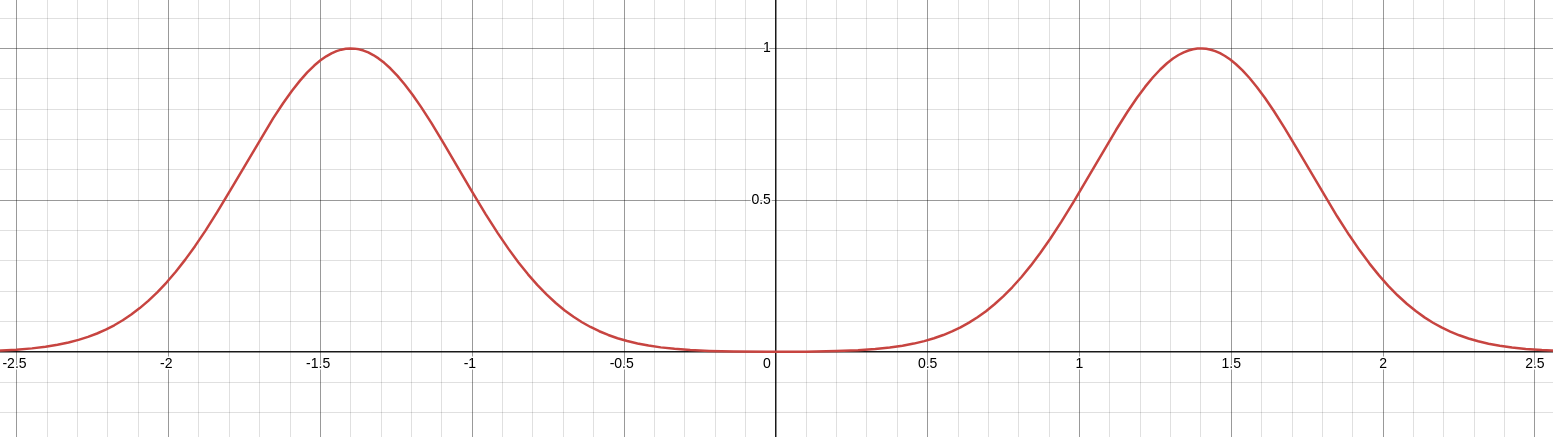
\includegraphics[width=0.9\textwidth]{fig/densi_spec_sym}
	\caption{Exemple de densité spectrale d'un signal réel ESP A 1,4}
	\label{fig:densi_spec_sym}
\end{figure}
\\
Même problème avec la covariance qui sera toujours nulle pour les signaux réels. De là en conclure que la fréquence instantanée de n'importe quel signal réel est toujours décorrélée du temps serait, pour le moins, insatisfaisant.
\\

Pour résoudre les problèmes lié à la fréquence moyenne et la largeur de bande, il suffirait de ne conserver que la partie positive du signal. On s'intéresserait alors au signal transformée $\SA{x}$ tel que :
\[\mathcal{F}\big[\SA{x}\big] = 2\one_{\R^+}\fou{x}\]
où $\one_E$ est la fonction indicatrice de l'ensemble $E$ et où le facteur 2 permet de conserver l'énergie du signal.
Avec la transformée de Fourier inverse, ce nouveau signal s'écrit alors :
\[\SA{x} = \mathcal{F}^{-1}\big[ 2\one_{\R^+}\fou{x} \big] = 2 \mathcal{F}^{-1}\big[\one_{\R^+}\big] * x\]
La transformée inverse de cette indicatrice (qui n'est autre que la fonction de Heavyside) n'est pas définie au sens classique, mais l'est au sens des distributions. Pour l'écrire, on introduit la distribution suivante :


\begin{definition}[valeur principale de Cauchy]\label{def:vp&Hilb}
	On appelle \emph{valeur principale de Cauchy} la distribution, notée $\vpC$, telle que :
	\begin{equation}
		\begin{aligned}
		\forall \varphi\in\mathcal{S}(\R),\qquad 
			\left\langle \vpC, \varphi \right\rangle 
			= \fint_0^t \frac{\varphi(t)}{t}dt 
			&\defeq \lim_{\varepsilon\lr0^+} \int_{-\infty}^{-\varepsilon} \frac{\varphi(t)}{t}dt + \int_{+\varepsilon}^{+\infty} \frac{\varphi(t)}{t}dt \\
			&= \int_0^{+\infty} \frac{\varphi(t) - \varphi(-t)}{t}dt
		\end{aligned}
	\end{equation}
	Ici $\mathcal{S}(\R)$ est l’espace de Schwartz des fonctions $C^\infty$ à décroissance rapide et la limite en $\varepsilon$ assure que l'intégrale (impropre) converge bien. Sa valeur est également appelée \emph{valeur principale} de l'intégrale. 
\end{definition}

La distribution vp$\frac{1}{x}$ est la valeur principale de la fonction inverse dans le sens où son produit avec l'identité donne 1 $\big(\left\langle id_\R \times \vpC, \varphi \right\rangle = \left\langle \vpC, id_\R \times\varphi \right\rangle=1\big)$ mais avec des propriétés d'intégration supplémentaires. Entre autre :


\begin{propriete}\label{prop:fou2vp}
	La transformée de Fourier de la valeur principale de Cauchy est donnée, au sens des distributions, par :
	\begin{equation}
		\mathcal{F} \left[\vpC \right]= -i \pi\, \sign{} 
	\end{equation}
	On en déduit la transformée de Fourier inverse :
	\begin{equation}
	\mathcal{F}^{-1}\big[ 2\one_{\R^+} \big] = \mathcal{F}^{-1}\big[ 1 + \sign \big] = \delta + \frac{i}{\pi} \vpC
	\end{equation}
\end{propriete}

	
\begin{demo}
	juste pour le plaisir. Par définition, la transformée de Fourier de la valeur principale est telle que,\\ $\forall \varphi\in\mathcal{S}(\R)$ :
	\begin{align*}
		\left\langle \mathcal{F} \left(\vpC \right), \varphi \right\rangle = \left\langle \vpC, \hat{\varphi} \right\rangle 
		&= \fint_\R \frac{\hat{\varphi}(\nu)}{\nu} d\nu \\
		&= \int_0^{+\infty} \frac{\hat{\varphi}(\nu) - \hat{\varphi}(-\nu)}{\nu} d\nu \\
		&= \int_0^{+\infty} \frac{1}{\nu} \left( \int_\R\varphi(t)e^{-2i\pi \nu t}dt - \int_\R\varphi(t)e^{2i\pi \nu t}dt \right)d\nu \\
		&= \int_0^{+\infty} \frac{1}{\nu}\int_\R\varphi(t)\big(e^{-2i\pi \nu t} - e^{2i\pi \nu t}\big)dt\, d\nu \\
		&= \int_0^{+\infty} \frac{1}{\nu}\int_\R-2i\varphi(t)\sin(2\pi \nu t)dt\, d\nu \\
		&= -2i\int_\R\varphi(t)\int_0^{+\infty} \frac{\sin(2\pi \nu t)}{\nu}d\nu\, dt
	\end{align*}
	En posant $u=2\pi\nu t\sign(t)$ (le signe de $t$ assure que l'on ait le même signe dans et hors du sin), on obtient :
	\begin{align*}
		\left\langle \mathcal{F} \left[\vpC \right], \varphi \right\rangle &= -2i\int_\R\varphi(t)\int_0^{+\infty} \sign(t)\frac{\sin(u)}{u}du\, dt \\
		&= -2i\int_\R\varphi(t)\frac{\pi}{2}\sign(t), dt \\
		&= \big\langle -i\pi\sign, \varphi \big\rangle
	\end{align*}
\end{demo}

\begin{definition}[Transformée en SA et de Hilbert]\label{def:transfo_sa&hilbert}
	On définie alors la \emph{transformée en signal analytique} (SA) du tout signal $x$ par l'application :
	\begin{equation}\label{eq:transfo_SA}
		\SA{x} = \sa{x} \defeq 2 x*\mathcal{F}^{-1}\big[\one_{\R^+}\big] :\ \begin{aligned} 
			\R \quad &\lr\qquad\quad \C \\	
			t\quad &\longmapsto\ x(t) + \frac{i}{\pi}\fint_\R \frac{x(s)}{t-s}ds
		\end{aligned}
	\end{equation}
	Par construction, on a bien $\mathcal{F}\big[\SA{x}\big] = 2\one_{\R^+}\fou{x}$, et on dira plus généralement de tout signal dont le spectre est réel positif que c'est un \emph{signal analytique}.
	\\
	L'intégral à droite de \eqref{eq:transfo_SA} est appelle \emph{transformée de Hilbert} du signal. Elle est notée :
	\begin{equation}\label{eq:transfo_Hilb}
		\mathcal{H}[x] :\ \begin{aligned} 
			\R \quad &\lr\qquad\quad \C \\	
			t\quad &\longmapsto\ \frac{1}{\pi}\fint_\R \frac{x(s)}{t-s}ds =  \frac{1}{\pi}\left(\vpC\right)*x
		\end{aligned}
	\end{equation}
\end{definition}

Par souci de commodité, plutôt que redéfinir tout le vocabulaire développé plus haut (fréquence moyenne, temps moyen, \etc) pour les signaux réel via la transformation $\mathcal{A}$, dans la suite du mémoire on travaillera directement avec $\SA{x}$. %^(et on verra que c'est essentiel).




\subsubsection{Propriétés et interprétations des signaux analytiques}\label{subsec:Bedrisan&AM-FM}


Dans les cas des signaux réels, la transformée de Hilbert est à valeur dans $\R$. Aussi, la transformée $\SA{x}$ à pour partie réelle $x$ et pour partie imaginaire $\mathcal{H}[x]$. Sous forme exponentielle, cela donne :
\[\SA{x}(t) = a(t)e^{i\phi(t)}\quad \Lr\quad \left\{\begin{aligned}x(t) &= a(t) \cos\phi(t) \\\mathcal{H}[x](t) &= a(t) \sin\phi(t)
\end{aligned}\right.\]
On obtient alors on décomposition de $x$ en une paire $(a,\phi)$ telle que discuté plus haut.

\begin{definition}[Amplitude et phase instantanée]\label{def:ampli&phase_instant}
	On définie ainsi l'\emph{amplitude instantanée} $a_x$ et la \emph{phase instantanée} $\phi_x$  de tout signal $x$ comme étant respectivement l'amplitude et la phase de $\SA{x}$ :
	\begin{align}\label{eq:ampli&phase_cano}
		a_x &= \big|\SA{x}\big|   &   \phi_x &= \arg\big(\SA{x}\big)
	\end{align}
\end{definition}

\begin{remarque}
	Il est important de noter que si un signal est présenté sous la forme  $\ x=a\cos\phi$, rien n'implique que $a$ et $\phi$ corresponde à l'amplitude et la phase instantanée du signal. Si ce n'est pas le cas, c'est que cette décomposition n'était ``pas la bonne'' en cela qu'elles ne s’interprètent pas comme l'on aimerait.
\end{remarque}

Pour comprendre comment cette transformation ``sélectionne'' la fréquence instantanée, détaillons le cas où $x$ s'écrit comme produit de deux signaux pures (\cref{fig:exemple_tSA_1/2}) :
\[x(t) = \cos (2\pi\nu_1t)\cos (2\pi\nu_2t)\]
\\
On montre sans mal\footnote{\itshape
	$\fou{x}$ est donné par 4 Diracs, en ne gardant que ce non nul sur $\R^+$ on obtient le spectre de $\SA{x}$ et il reste plus qu'à inverser la transformée de Fourier.}
que si $\nu_1\geq\nu_2$, alors la transformée en SA de $x$ s'écrit :
\[\SA{x} = \cos \left(2\pi\nu_2 t\right) e^{2\i\pi\nu_1 t}\]

\begin{figure}[h]\centering
	%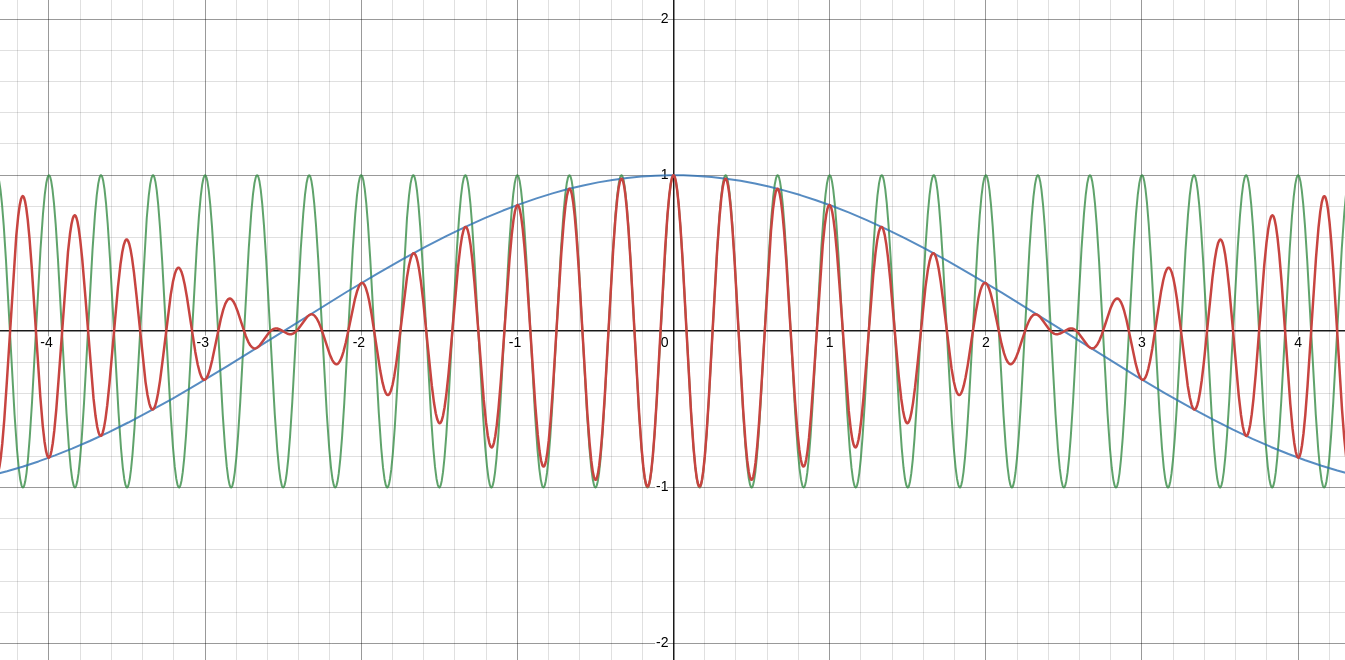
\includegraphics[width=0.48\textwidth]{fig/ex SA - 11.png}\hfill
	%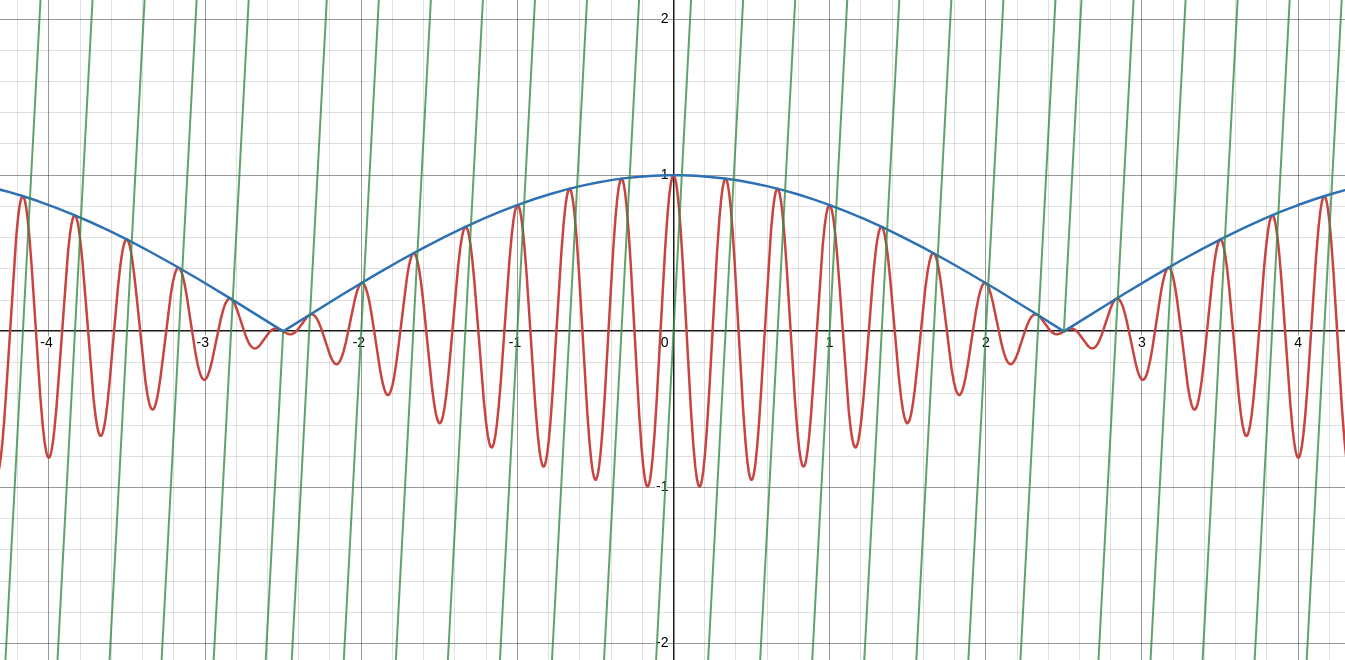
\includegraphics[width=0.48\textwidth]{fig/ex SA - 12.png}
	\caption{Représentation graphique du signal $x$ (rouge) avec $\nu_1=3$ et $\nu_2=0.1$. Sur l'image de gauche, avec signaux de fréquences pures (bleu et vert). Sur l'image de droite, avec son amplitude (bleu) et sa phase instantanée (vert). Les discontinuités de la phase sont dû à l'arrondi à $2\pi$  près de l'argument de $\SA{x}$ et à la façon dont il est calculé lorsque le signal s'annule (mise à 0). Voir \href{https://www.desmos.com/calculator/gcedcdfkhr}{ici} pour un graphique dynamique.}
	\label{fig:exemple_tSA_1/2}
\end{figure}
\noindent
Le signal $\SA{x}$ n'est ici pas sous forme exponentielle à proprement parler puisque le cosinus peut être négatif (pour s'y ramener, il suffit de passer le cos en valeur absolue et d'ajouter $\pi$ à l'argument lorsque nécessaire) mais l’avantage de cette forme est qu'elle fait clairement apparaître les fréquences $\nu_{1,2}$. En particulier, la fréquence instantanée du signal est la plus grandes des deux fréquences $\nu_1$ et $\nu_2$. La plus petite, elle, se retrouve dans l'amplitude. 
\\
Ce résultat est rassurant en cela qu'il est plus naturel de voir le cosinus de basse fréquence comme modulant celui de haute fréquence que l'inverse comme on le voit sur la première image de la figure \ref{fig:exemple_tSA_1/2}. 
\\
Aussi, en mettant les hautes fréquences du signal dans la fréquence instantanée, on s'assure de limiter les variations de l'amplitude. Cela apporte bien plus de contrainte en terme de décomposition $(a_x,\phi_x)$, en cela qui si l'inverse étant vrai, alors toute les fréquences pourrait être envoyé dans l'amplitude, ce qui laisserait la phase invariante.
\\

Cela étant dit, lorsque l'on fait varier $\nu_1$ et $\nu_2$, le résultat n'est pas toujours si intuitif. C'est notamment le cas lorsque les deux deviennent de plus en plus proche :

\begin{figure}[h]\centering
	%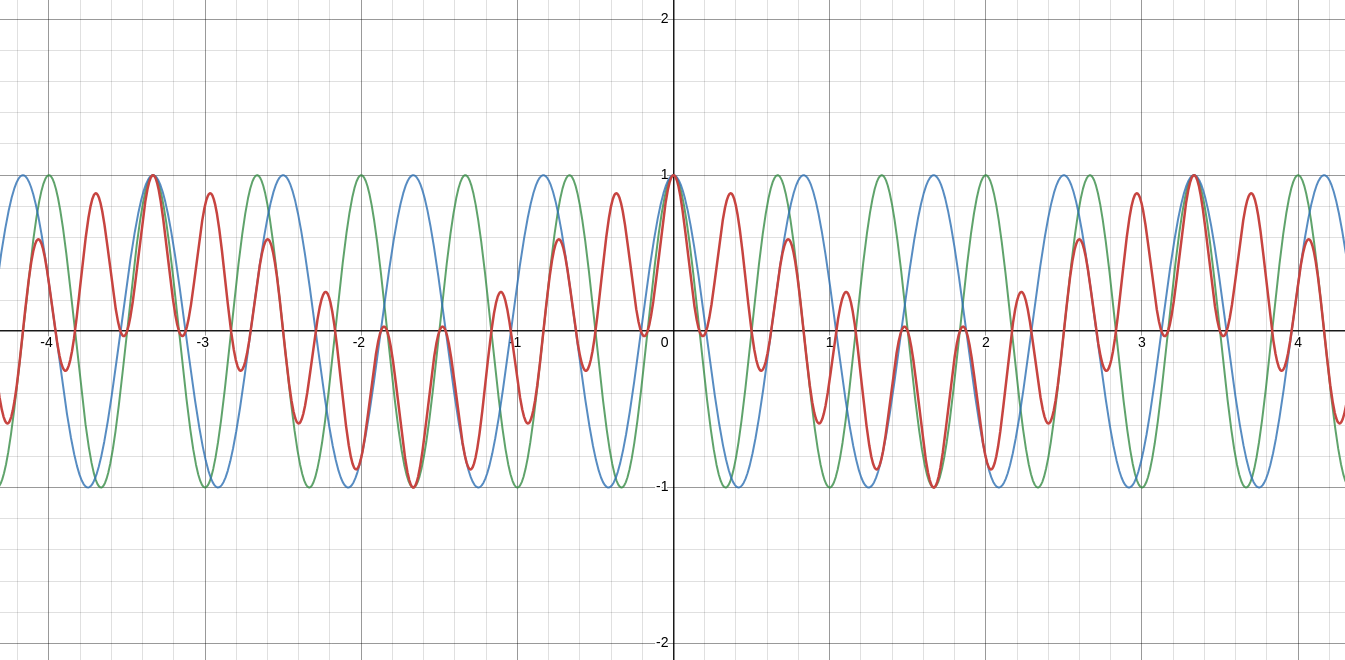
\includegraphics[width=0.48\textwidth]{fig/ex SA - 21.png}\hfill
	%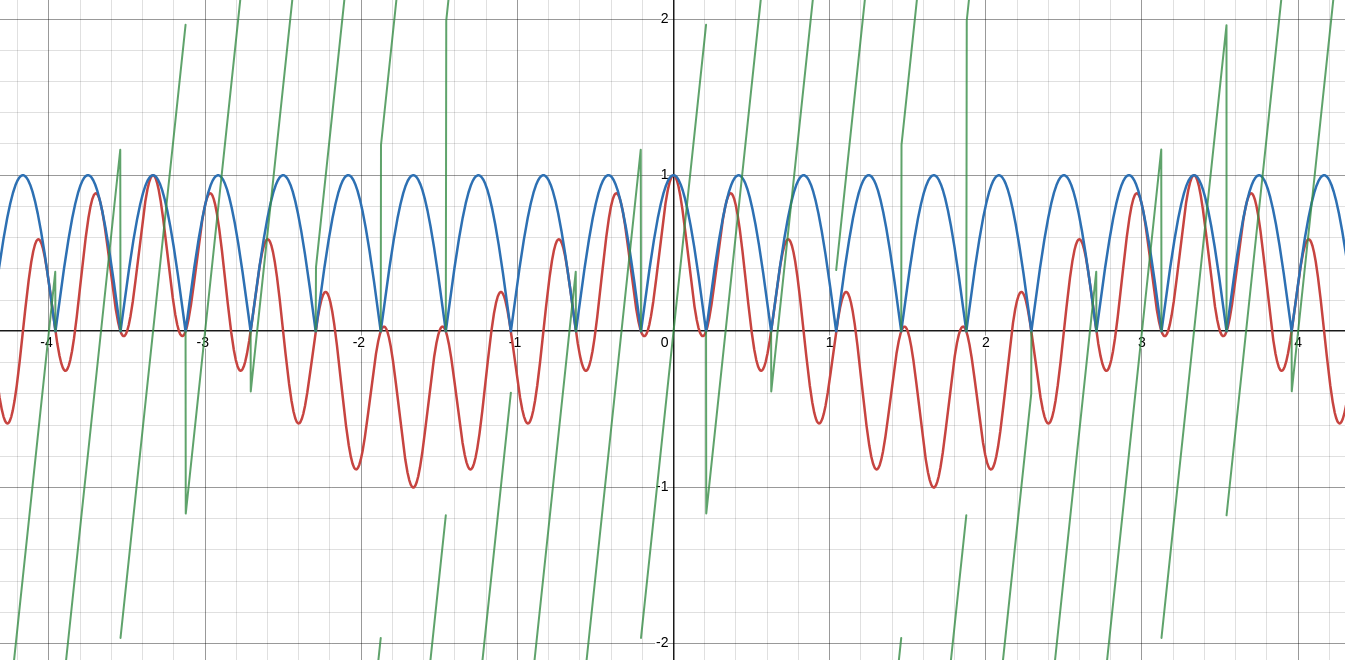
\includegraphics[width=0.48\textwidth]{fig/ex SA - 22.png}
	\caption{Idem que pour la figure \ref{fig:exemple_tSA_1/2} précédente, avec cette fois $\nu_1=1.5$ et $\nu_2=1.3$.}
	\label{fig:exemple_tSA_2/2}
\end{figure}

Pour comprendre pourquoi l'amplitude ne fait pas ce qu'on attendrait d'elle, on introduit le théorème de Bedrosian :

\begin{theoreme}[de Bedrosian]\label{theo:2Bedrosian}
	Dans sa formulation la plus générale, le théorème de Bedrosian énonce que donnée si deux fonctions $f,g\in L^2(\R)$ sont telles l'une des trois assertions suivantes est vraie :
	\newline
	\begin{enumerate}[label=\textit{\arabic*}. ]
		
		\item $\exists \lambda\in\R^+\ |\ \supp \fou{f} \subset [-\lambda, +\infty[,\ \supp \fou{g} \subset [\lambda, +\infty[$\label{item:1condi_theo2Bedrosian}
		
		\item $\exists \lambda\in\R^+\ |\ \supp \fou{f} \subset ]-\infty, \lambda],\ \supp \fou{g} \subset ]-\infty,-\lambda]$ \label{item:2condi_theo2Bedrosian}
		
		\item $\exists (\lambda_1,\lambda_2)\in \R^+\times\R^+ \setminus\{(0,0)\}\ |\ \supp \fou{f} \subset [-\lambda_1, \lambda_2],\ \supp \fou{g} \subset \R\setminus[-\lambda_2,\lambda_1]$
		
	\end{enumerate}
	alors la transformée de Hilbert de leur produit est donnée par la formule (voir \cite{wang_simple_2009} pour une démonstration) :
	\begin{equation}\label{eq:2Bedrosian}
		\hilb{fg} = f\hilb{g}
 	\end{equation}
\end{theoreme}

\begin{corollaire}\label{coro:AM-FM}
	Dans le cas d'un signal réel, suivant la \cref{def:ampli&phase_instant} on peut écrire \newline $x=a_x\cos\circ\phi_x$.
	Comme $a_x$ et $\phi_x$ sont réels, seule la \ref{item:2condi_theo2Bedrosian} condition du théorème de Bedrosian peut être satisfaite pour peu que $\lambda_1=\lambda_2$.
	\\
	Ainsi, à condition que $a_x\in L^2(\R)$, $\cos\phi_x\in L^2(\R)$ et qu'il existe $\lambda\in\R^{+_*}$ tel que :
	\[\supp \Fou{a_x} \subset [-\lambda, \lambda],\quad \supp \Fou{\cos\phi_x} \subset \R\setminus[-\lambda,\lambda]\]
	 Alors on a :
	\begin{align*}
		\hilb{x} &= a_x\hilb{\cos(\phi_x)}  &  &\text{et}  &  \hilb{\cos(\phi_x)} = \sin(\phi_x)
	\end{align*}
\end{corollaire}



\section{Généralisation aux signaux multivariés}\label{sec:sign_multivar}

\begin{definition}[Signal multivarié]\label{def:signal_multivar}
	Un \emph{signal multivarié}, ou \emph{$n-$varié}, est un vecteur composé de $n\in\N^*$ signaux $x_i$. Si $n=2$, alors on parle de signal \emph{bivarié}.
	\\
	Dans la continuité de ce qui à été dit dans la \cref{subsec:transfo_SA}, dans le cas des signaux réels, on s'intéressera au vecteur composé des transformées en SA (eq. \ref{eq:transfo_SA}, déf. \ref{def:transfo_sa&hilbert}) des $x_i$.
	\textbf{Au moins dans toute cette \namecref{sec:sign_multivar}}, un tel signal sera noté :
	\[\sa{x}(t)\ :\quad \begin{aligned} 
		\R\quad &\lr\qquad \C^n \\t\quad &\longmapsto\ \begin{pmatrix} \mathcal{A}[x_1] \\ 
			\mathcal{A}[x_2] \\ \vdots \\ \mathcal{A}[x_n] \end{pmatrix}
	\end{aligned} \]
	On supposera que chaque composante $x_i$ de $\bf{x}$ aura autant de régularité et de condition d'intégrabilité que nécessaire \textbf{(il vaudra préciser lesquelles à un moment)}.
\end{definition}

Le fait que $\bf{x}$ soit à valeur dans $\C^n$ impose un choix naturel de d'amplitude instantanée : sa norme. L'on notera alors dans tout la suite (sauf précision) :
\[\forall t\in\R,\qquad 
	\bf{x}(t) = a(t)\begin{pmatrix} a_1(t)e^{i\phi_1(t)} \\ a_2(t)e^{i\phi_2(t)} \\ \vdots \\ a_n(t)e^{i\phi_n(t)}
\end{pmatrix} \qquad\text{ avec }\qquad \big\|(a_i)_{1\leq i\leq n}\big\|=1,\quad a\geq 0
%a(t)e^{i\phi(t)}\begin{pmatrix} a_1(t)e^{i\psi_1(t)} \\ a_2(t)e^{i\psi_2(t)} \\ \vdots \\ a_n(t)e^{i\psi_n(t)}\end{pmatrix}
\]
\\
Le choix de la phase instantanée, en revanche, n'est pas plus commode. Si l'on cherche à écrire $\bf{x}$ sous la forme :
\[a(t)e^{i\phi(t)}\begin{pmatrix} a_1(t)e^{i\psi_1(t)} \\ a_2(t)e^{i\psi_2(t)} \\ \vdots \\ a_n(t)e^{i\psi_n(t)}
\end{pmatrix}\]
alors n'importe quel choix de $\phi$ est valable, il suffit que $\ \psi_i = \phi_i-\phi$.



\subsection{Phase et fréquence instantanée de signal multivarié }\label{subsec:param_instant_nvar}

Afin de contraindre ce choix, on s'inspire propriétés de la phase instantanée vu plus tôt pour en déduire deux approches :
\begin{itemize}
	\item D'une part, l'espérance de la fréquence instantanée (ici vu comme dérivée à $2\pi$ près de la phase\footnote{\itshape
		La pertinance de cette définition dans le cas multivarié sera discuté plus loin})
	doit donnée la fréquence moyenne au sens de Fourier, eq. \eqref{eq:esp_freq}.
	
	\item D'autre part, les conditions d'interprétation de la décomposition $(a_x,\phi_x)$, \cref{theo:2Bedrosian}, exige que les hautes fréquences du signal se retrouve dans la phase.
\end{itemize}

Pour cela on introduit les notations utiles au cas multivarié :
\begin{definition}[densité d’énergie]\label{def:densi_dE-mv}
Étant donné un signal multivarié $\bf{x}=(x_i)_{1\leq i\leq n}$, les densités d'énergie de chaque composante $x_i$  sont notées :
\begin{align}\label{eq:densi_dEi}
	\densit_i\ &:\quad \begin{aligned}\R\ &\lr\quad \R^+ \\ t\ &\longmapsto\ \big|x_i(t)\big|^2 = a(t)^2 a_i(t)^2 \end{aligned}  
	&
	\densis_i\ &:\quad \begin{aligned}\R\ &\lr\quad \R^+ \\ \nu\ &\longmapsto\ \big|\fou{x}_i(\nu)\big|^2 \end{aligned}
\end{align}
Et les densités d'énergies associées au signal $\bf{x}$ complet :
\begin{align}\label{eq:densi_dE-mv}
	\densit\ &:\quad \begin{aligned}\R\ &\lr\quad \R^+ \\ t\ &\longmapsto\ \big\|\bf{x}(t)\big\|^2 = \sum_{i=1}^n \densit_i(t) \end{aligned}  
	&
	\densis\ &:\quad \begin{aligned}\R\ &\lr\quad \R^+ \\ \nu\ &\longmapsto\ \big\|\fou{\bf{x}}(\nu)\big\|^2 = \sum_{i=1}^n \densis_i(t) \end{aligned}	
\end{align}
\end{definition}

La première approche, inspiré de \cite{cano_mathematical_2022} consiste donc de reprendre le ``calculation trick'' \eqref{eq:moment_f}, pour en déduire la fréquence moyenne
\begin{align*}
	\esp[\densis]{\nu} = \int_\R \nu\densis(\nu)d\nu &= \int_\R \nu\sum_{i=1}^n \densis_i(\nu) d\nu \\
		 &= \sum_{i=1}^n\esp[\densis_i]{\nu} \\
		 &= \sum_{i=1}^n\frac{1}{2\pi}\int_\R \phi_i'(t)\densit_i(t)dt \\
		 &= \frac{1}{2\pi}\int_\R a(t)^2\sum_{i=1}^n\phi_i'(t)a_i(t)^2 dt 
		 \\ &= \frac{1}{2\pi} \esp[\densit]{\sum_{i=1}^n \phi_i'{a_i}^2}
\end{align*}
\\
Ce qui mène à une première définition de la phase instantanée :
\begin{equation}\label{eq:phas_inst_v1}
	\phi = \int \sum_{i=1}^n \phi_i'(s){a_i}(s)^2ds 
	= \sum_{i=1}^n \int \phi_i'(s){a_i}(s)^2ds 
	%= \sum_{i=1}^n \esp[\nicefrac{\densit_i}{\densit}]{\phi_i'}
\end{equation}
\\

La seconde approche, fortement inspirée par les travaux de Lilly \& Olhede  \cite{lilly_analysis_2012}, se base sur la discussion autour du théorème Bedrisan sur la séparation haute-basse fréquence du signal $\bf{x}$ (\cref{subsec:Bedrisan&AM-FM}). Pour cela, l'on commence par faire apparaître la phase $\phi$ --- pour l'instant inconnue --- en écrivant $\bf{x}$ sous la forme :
\[\forall t\in\R,\qquad \bf{x}(t) = e^{i\phi(t)} e^{-i\phi(t)} \bf{x}(t) \defeq e^{i\phi(t)} \Tilde{\bf{x}}(t)\]
\\
Si $\phi$ est bien choisie, alors $\Tilde{\bf{x}}$ contient les informations associées à l'amplitude et la polarisation de $\bf{x}$. Or, la phase doit contenir les hautes fréquences du signal. 
Pour s'en assurer on demande, à l'inverse, que les basses fréquences du signal soit données par $\Tilde{\bf{x}}$ en limitant ces variations. En clair, $\phi$ doit être choisi de sorte à minimiser la dérivée $\Tilde{\bf{x}}'$ :
\[\forall t\in\R,\qquad \phi(t) = \argmin{\alpha(t)}{\big\|\Tilde{\bf{x}}'(t)\big\|_2}^2 = \argmin{\alpha(t)}{\Big\|e^{-i\alpha}\big(\bf{x}' - i\alpha'\bf{x}\big)\Big\|_2}^2 = \argmin{\alpha(t)}{\big\|\bf{x}' - i\alpha'\bf{x}\big\|_2}^2\]
\\
La contrainte ne dépendant que de la dérivée $\alpha'$, on se ramène à :
\[\min_{\alpha(t)}{\|\Tilde{\bf{x}}'(t)\|_2}^2 = \min_{\alpha'(t)}{\big\|\bf{x}'(t) - \alpha'(t) \bf{x}(t)\big\|_2}^2\]
\\
En rappelant que $\frac{d}{dx}{\big\|f(x)\big\|_2}^2 = 2\Re e\big\langle f(x), f'(x)\big\rangle$, il vient que ce minimum\footnote{\itshape
	L'extremum obtenu est l'unique minimum puisque $t\longmapsto \|at + b\|^2$ est strictement convexe pour $a\neq0$.}
 est atteint par $\phi'(t)$ à condition que :
\begin{align*}
	\frac{d}{d\phi'}{\big\| \bf{x}' - i\phi' \bf{x}\big\|_2}^2 = 0 \quad \Llr\quad
		0 &= 2\Re e\left\langle  \bf{x}' - i\phi' \bf{x} ,  \frac{d}{d\phi'}\big(\bf{x}' - i\phi' \bf{x}\big)\right\rangle \\
		&= 2\Re e\big\langle  \bf{x}' - i\phi' \bf{x} ,  - i \bf{x}\big\rangle \\
		&= 2\Re e\Big(i\big\langle  \bf{x}' ,  \bf{x}\big\rangle\Big) + 2\phi'\Re e\big\langle   \bf{x} ,  \bf{x}\big\rangle\\
		&= -2\Im m\big\langle  \bf{x}' ,  \bf{x}\big\rangle + 2\phi'{\| \bf{x}\|_2}^2
\end{align*}
Ainsi :
\begin{align}\label{eq:phas_inst_v2}
	\phi' &= \frac{\Im m\big\langle  \bf{x}' ,  \bf{x}\big\rangle}{{\| \bf{x}\|_2}^2} = \frac{-\Im m\big\langle  \bf{x},  \bf{x}'\big\rangle}{{\| \bf{x}\|_2}^2}  &  &\text{et}  &  \phi &= -\Im m\int \frac{\big\langle \bf{x}(s) , \bf{x}'(s) \big\rangle}{\|\bf{x}(s)\|^2} ds
\end{align}
\\
Ce qui, sous forme exponentiel, se réécrit :
\begin{align*}
	-\Im m\frac{\big\langle \bf{x}(t) , \bf{x}'(t) \big\rangle}{\|\bf{x}(t)\|^2} &= -\Im m\frac{1}{a(t)^2} \sum_{i=1}^n a(t)a_i(t)e^{i\phi_i(t)}\congu{\Big( \big(aa_i\big)'(t) +a(t)a_i(t)i\phi_i'(t)\Big)e^{i\phi_i(t)}} \\
	&= -\Im m\frac{1}{a(t)^2} \sum_{i=1}^n a(t)a_i(t)\big(aa_i\big)'(t) -ia(t)^2a_i(t)^2\phi_i'(t) \\
	&= -\frac{1}{a(t)^2} \sum_{i=1}^n -a(t)^2a_i(t)^2 \phi_i'(t) \\
	&= \sum_{i=1}^n a_i(t)^2 \phi_i'(t)
\end{align*}
Soit la même expression que \eqref{eq:phas_inst_v1} obtenue par le premier raisonnement.
\\
\begin{remarque}[Notation à reprendre ($aa_i$)]
	Toujours avec les mêmes notations, une conséquence de l'\cref{eq:phas_inst_v2} est que les fréquences $\psi_i$ restantes sont de moyenne nulle dans le sens où :
	\begin{equation}\label{eq:sum_esp_null}
		\sum_{i=1}^n \int \psi_i'(s){a_i}(s)^2ds =0
	\end{equation}
	Moralement, ca revient juste à dire qu'en définissant $\phi$ suivant Lilly, on a ôté au $\psi_i$ la phase moyenne pondérée et donc, tout naturellement, les nouvelles phase individuelles $\psi_i$ sont centrés (à la même pondération près). Cela revient peut ou prou à la première \cref{eq:phas_inst_v1}.
	\\
	Pour le montrer, il suffit de refaire le calcul de la phase instantanée :
	\begin{align*}
		\big\langle \bf{x}(t) \,|\, \dot{\bf{x}}(t) \big\rangle &= \Big\langle \Big(a_i(t)e^{i(\phi(t)+\psi_i(t))}\Big)_i \,\Big|\, \Big(\big(a_i'(t)+i\big( \phi(t)+\psi_i(t) \big)a_i(t)\big)e^{i(\phi(t)+\psi_i(t))}\Big)_i \Big\rangle \\
		&= \sum_i a_i(t) \Big(a_i'(t)-i\big(\phi'(t) + \psi_i'(t)\big)a_i(t)\Big) \\
		&= \sum_i a_i(t)a_i'(t)-i\sum_i \big(\phi'(t) + \psi_i'(t)\big)a_i(t)^2 \\
		&= \sum_i a_i(t)a_i'(t)-i \phi'(t)\sum_ia_i(t)^2  - i\sum_i \psi_i'(t)a_i(t)^2 \\
		&= \sum_i a_i(t)a_i'(t)-i \phi'(t)\big\|a(t)\big\|^2  - i\sum_i \psi_i'(t)a_i(t)^2
	\end{align*}
	\\
	Ce qui mène à :
	\begin{align*}
		\phased(\bf{x},t_0,t) &= \int_{t_0}^t \frac{\varphi'(s)\big\|a(s)\big\|^2}{\big\|a(s)\big\|^2} ds  + \sum_i\int_{t_0}^t \frac{\varphi_i'(s)a_i(s)^2}{\big\|a(s)\big\|^2} ds \\
		&=\phased(\bf{x},t_0,t)  + = \sum_{i=1}^n \int \psi_i'(s){a_i}(s)^2ds 
	\end{align*}
\end{remarque}




\subsection{Cas bivarié et trivarié}

\subsubsection{Bivarié}

\begin{proposition}[phases de signal AM--FM--PM]\label{prop:phased/t_2var}
	\'Etant donné un signal bivarié AM--FM--PM $\bf{x}$, \ie~de la forme :
	\begin{equation}\label{eq:exp_elliptik_2var}
		\bf{x} = ae^{i\varphi} R_{\theta} \begin{pmatrix} \cos\chi \\ -i\sin\chi \end{pmatrix} 
			= a(t)e^{i\varphi} \begin{pmatrix} \cos\theta \cos\chi + i\sin\theta \sin\chi \\ \sin\theta \cos\chi - i\cos\theta \sin\chi \end{pmatrix}
	\end{equation}
	\\
	la phase dynamique de $\bf{x}$ est donnée par :
	\begin{equation}\label{eq:phased_2var}
		\phased(\bf{x}, t_0,t) = \int_{t_0}^t \dot{\varphi}(s) + \dot{\theta}(s) \sin2\chi(s) ds = \varphi(t) -\varphi(t_0) + \int_{t_0}^t\dot{\theta}(s) \sin2\chi(s) ds
	\end{equation}
	\\
	Soit une différence de phase $\varphi$ mais avec un terme en plus. Donc $\varphi$ ne doit (\textbf{doit?}) pas être interpréter comme la phase instantanée du signal, où du moins pas au sens donnée dans la \cref{subsec:param_instant_nvar}.
	\\
	La phase totale, elle, s'écrit :
	\begin{equation}\label{eq:phaset_2var}
		\begin{aligned}
			\phaset(\bf{x},t_0,t) = \arg\big\langle \bf{x}(t), \bf{x}(t_0)\big\rangle &= \varphi(t)-\varphi(t_0) + \arg\Big(\cos\Delta\theta \cos\Delta\chi + i\sin\Delta\theta \sin\big(\chi(t_0)+\chi(t)\big)\Big) \\
			&= \varphi(t)-\varphi(t_0) + \arctan\left(\tan\Delta\theta \frac{ \tan\chi(t_0)+\tan\chi(t)}{1 + \tan\chi(t_0)\tan\chi(t)}\right)
		\end{aligned}
	\end{equation}
	ou $\ \Delta y = y(t) - y(t_0)\ $ pour $\ y=\varphi,\theta,\chi$. \textbf{(adapte signe démo)}
\end{proposition}

\begin{demo}[de la \cref{prop:phased/t_2var}]
	Par souci de lisibilité, on note $\mathcal{U} = R_{\theta} \begin{pmatrix} \cos\chi \\ -i\sin\chi \end{pmatrix}$ de sorte que la dérivée de $\bf{x}$ s'écrive :
	\begin{align*}
		\dot{\bf{x}} 
			&= \dot{a}e^{i\varphi}\mathcal{U} + ia\dot{\varphi}e^{i\varphi} \mathcal{U} + ae^{i\varphi}\dot{\theta}\begin{pmatrix} -\sin\theta \cos\chi + i\cos\theta \sin\chi \\ \cos\theta \cos\chi + i\sin\theta \sin\chi \end{pmatrix} + ae^{i\varphi}\dot{\chi}\begin{pmatrix} -\cos\theta \sin\chi + i\sin\theta \cos\chi \\ -\sin\theta \sin\chi - i\cos\theta \cos\chi \end{pmatrix} \\
			&= \dot{a}e^{i\varphi}\mathcal{U} + ia\dot{\varphi}e^{i\varphi} \mathcal{U} + ae^{i\varphi}\dot{\theta}\begin{pmatrix} 0 & -1 \\ 1 & 0 \end{pmatrix}\mathcal{U} + ae^{i\varphi}\dot{\chi}\begin{pmatrix} 0 & i \\ -i & 0 \end{pmatrix}\congu{\mathcal{U}}
	\end{align*}
	\\
	Le produit hermitien $\langle \bf{x}, \dot{\bf{x}}\rangle$ s'écrit alors :
	\begin{align*}
		\langle \bf{x}, \dot{\bf{x}}\rangle 
			&= \left\langle ae^{i\varphi}\mathcal{U}, \dot{a}e^{i\varphi}\mathcal{U} + ia\dot{\varphi}e^{i\varphi} \mathcal{U} + ae^{i\varphi}\dot{\theta}\begin{pmatrix} 0 & -1 \\ 1 & 0 \end{pmatrix}\mathcal{U} + ae^{i\varphi}\dot{\chi}\begin{pmatrix} 0 & i \\ -i & 0 \end{pmatrix}\congu{\mathcal{U}}\right\rangle \\
			&= \left\langle a\mathcal{U}, \dot{a}\mathcal{U} + ia\dot{\varphi} \mathcal{U} + a\dot{\theta}\begin{pmatrix} 0 & -1 \\ 1 & 0 \end{pmatrix}\mathcal{U} + a\dot{\chi}\begin{pmatrix} 0 & i \\ -i & 0 \end{pmatrix}\congu{\mathcal{U}}\right\rangle \\
			&= a\dot{a} \big\langle \mathcal{U}, \mathcal{U}\big\rangle  - ia^2\dot{\varphi} \big\langle \mathcal{U}, \mathcal{U}\big\rangle  + a^2\dot{\theta}\left\langle \mathcal{U}, \begin{pmatrix} 0 & -1 \\ 1 & 0 \end{pmatrix}\mathcal{U}\right\rangle + ia^2\dot{\chi}\left\langle \mathcal{U}, \begin{pmatrix} 0 & -1 \\ 1 & 0 \end{pmatrix}\congu{\mathcal{U}}\right\rangle
	\end{align*}
	où les deux derniers produits hermitiens donnent :
	\begin{align*}
		\left\langle \mathcal{U}, \begin{pmatrix} 0 & -1 \\ 1 & 0 \end{pmatrix}\mathcal{U}\right\rangle &= -\mathcal{U}_1\congu{\mathcal{U}_2} + \mathcal{U}_2\congu{\mathcal{U}_1} \\
		&= 2i\Im m\big(\congu{\mathcal{U}_1} \mathcal{U}_2\big) \\
		&= 2i\Im m\big(\cos\theta \cos\chi - i \sin\theta \sin\chi \big) \big( \sin\theta \cos\chi - i \cos\theta \sin\chi \big) \\
		&= 2i\big(-\cos^2\theta \cos\chi \sin\chi - \sin^2\theta \sin\chi \cos\chi \big) \\
		&= -2i\big( \cos\chi \sin\chi + \sin\chi \cos\chi \big) \\
		&= -i\sin2\chi 
		\\ \\
	\left\langle \mathcal{U}, \begin{pmatrix} 0 & -1 \\ 1 & 0 \end{pmatrix}\congu{\mathcal{U}}\right\rangle &= -\mathcal{U}_1\mathcal{U}_2 + \mathcal{U}_2\mathcal{U}_1 = 0
	\end{align*}
	\\
	D'où, sachant que $\ \|\bf{x}\|^2=a^2\ $ et $\ \|\mathcal{U}\|=1$, la formule :
	\begin{align*}
		-\frac{\Im m\big\langle \bf{x},\dot{\bf{x}}\big\rangle}{\|\bf{x}\|^2} &= -\frac{1}{a^2}\Im m\Big(a\dot{a} \big\langle \mathcal{U}, \mathcal{U}\big\rangle  - ia^2\dot{\varphi} \big\langle \mathcal{U}, \mathcal{U}\big\rangle - ia^2\dot{\theta} \sin2\chi \Big) \\
		&= \frac{1}{a^2} \Big( a^2\dot{\varphi} \|\mathcal{U}\|^2 + a^2\dot{\theta} \sin2\chi \Big) \\
		&= \dot{\varphi} + \dot{\theta} \sin2\chi
	\end{align*}
	%\begin{pmatrix} \cos\theta \cos\chi + i\sin\theta \sin\chi \\ \sin\theta \cos\chi - i\cos\theta \sin\chi \end{pmatrix}
	\\
	
	Pour la phase totale, on note cette fois $\mathcal{V} = \begin{pmatrix} \cos\chi \\ -i\sin\chi \end{pmatrix}$ et on a :
	\begin{align*}
		\big\langle \bf{x}(t_0), \bf{x}(t)\big\rangle &= \Big\langle a(t_0)e^{i\varphi(t_0)}R_{\theta(t_0)}\mathcal{V}(t_0), a(t)e^{i\varphi(t)}R_{\theta(t)}\mathcal{V}(t) \Big\rangle \\
		&= a(t_0)e^{i\varphi(t_0)}a(t)e^{-i\varphi(t)}\Big\langle R_{\theta(t_0)}\mathcal{V}(t_0), R_{\theta(t)}\mathcal{V}(t) \Big\rangle \\
		%&= a(t_0)a(t)e^{i(\varphi(t_0)-\varphi(t))}\Big\langle \mathcal{V}(t_0), R_{\theta(t_0)}^{-1}R_{\theta(t)}\mathcal{V}(t) \Big\rangle \\
		&= a(t_0)a(t)e^{i(\varphi(t_0)-\varphi(t))}\Big\langle \mathcal{V}(t_0), R_{\theta(t)- \theta(t_0)}\mathcal{V}(t) \Big\rangle
	\end{align*}
	Pour alléger les notations, on note $\ \Delta y =y(t)-y(t_0)$, $\ y_1=y(t_0)\ $ et $\ y_2=(t)\ $ pour $\ y=\varphi,\theta,\chi$. Le produit hermitien à droite s'écrit alors :
	\begin{align*}
		\Big\langle \mathcal{V}(t_0), R_{\Delta\theta}\mathcal{V}(t) \Big\rangle &= \begin{pmatrix} \cos\chi_1 & -i\sin\chi_1 \end{pmatrix}  \begin{pmatrix} \cos\Delta\theta \cos\chi_2 - i\sin\Delta\theta \sin\chi_2 \\ \sin\Delta\theta \cos\chi_2 + i\cos\Delta\theta \sin\chi_2 \end{pmatrix} \\
		&= \cos\chi_1\Big(\cos\Delta\theta \cos\chi_2 - i\sin\Delta\theta \sin\chi_2\Big) - i\sin\chi_1\Big(\sin\Delta\theta \cos\chi_2 + i\cos\Delta\theta \sin\chi_2\Big) \\
		&= \cos\Delta\theta \Big(\cos\chi_1 \cos\chi_2 + \sin\chi_1 \sin\chi_2\Big) - i\sin\Delta\theta \Big( \cos\chi_1 \sin\chi_2 + \sin\chi_1\cos\chi_2\Big) \\
		&= \cos\Delta\theta \cos\Delta\chi - i\sin\Delta\theta \sin(\chi_1+\chi_2)
	\end{align*}
\end{demo}




\subsubsection{Trivarié}

\begin{itemize}
	\item Version de Lilly \cite{lilly_modulated_2011}
	\begin{equation}
		\begin{aligned}
			\sa{\bf{x}}(t) &= e^{i\phi(t)} R_1\big(\alpha(t)\big)\ R_3\big(\beta(t)\big)\ R_1\big(\theta(t)\big)\begin{pmatrix}
				a(t) \\ -ib(t) \\ 0
			\end{pmatrix} \\
			&= a(t)e^{i\phi(t)} R_1\big(\alpha(t)\big)\ R_3\big(\beta(t)\big)\ R_1\big(\theta(t)\big)\begin{pmatrix}
				\cos\chi(t) \\ -i\sin\chi(t) \\ 0
			\end{pmatrix}
		\end{aligned}
	\end{equation}
	
	\begin{align*}
		&\text{avec : }  &  
		R_1(\theta) &= \begin{pmatrix}
			1 & 0 & 0 \\ 0 & \cos\theta & -\sin\theta \\ 0 & \sin\theta & \cos\theta
		\end{pmatrix}  &  
		R_3(\theta) &= \begin{pmatrix}
			\cos\theta & -\sin\theta & 0 \\ \sin\theta & \cos\theta & 0 \\ 0 & 0 & 1 
		\end{pmatrix}
	\end{align*}
	
	Donc une amplitude / phase instantanée $A$ / $\phi$ et une polarisation instantanée d'ellipse paramétrée par $\chi$ et orientée par la rotation $R_1R_3R_1$.
	
	\item On note d'abord que (Lefevre \cite{lefevre_polarization_2021}) :
	\[\begin{pmatrix}
		\cos\chi(t) \\ -i\sin\chi(t) \\ 0
	\end{pmatrix} = \begin{pmatrix}
		\cos\chi(t) & i\sin\chi(t) & 0 \\ -i\sin\chi(t) & \cos\chi(t) & 0 \\ 0 & 0 & 1
	\end{pmatrix}\begin{pmatrix}
	1 \\ 0 \\ 0
	\end{pmatrix}\]
	Ce qui, en terme de matrice de Gall-man $(\lambda_i)$ (généralisation de la base de Pauli à $\U(3)$), devient :
	\begin{align*}
		\sa{\bf{x}}(t) &= a(t)e^{i\phi(t)} R_1\big(\alpha(t)\big)\ R_3\big(\beta(t)\big)\ R_1\big(\theta(t)\big)\begin{pmatrix}
			\cos\chi(t) \\ -i\sin\chi(t) \\ 0
		\end{pmatrix} \\
		&= a(t)e^{i\phi(t)} e^{i\alpha \lambda_7} e^{i\beta \lambda_3} e^{i\theta \lambda_7} e^{-i\chi \lambda_1}\begin{pmatrix}
			1 \\ 0 \\ 0
		\end{pmatrix}
	\end{align*}
	
	
\end{itemize}





\subsection{Généralisation de ces formules au cas $\bf{n-}$varié}

\begin{proposition}[phase de signal AM--FM--PM $n$-varié]\label{prop:phased_nvar}
	La formule \ref{eq:phased_2var} de la \cref{prop:phased/t_2var} ce généralise très bien à plus haute dimension. En écrivant $\bf{x}$ sous la forme :
	\begin{align}\label{eq:exp_elliptik_nvar}
		\bf{x}(t) &= a(t)e^{i\varphi} R_{\Theta(t)} \mathcal{V}(t)  &  \text{où }\ R_{\Theta(t)} \in\SO_n(\R)  \ \text{ et }\  \mathcal{V}(t) &= \begin{pmatrix} \cos\chi(t) \\ -i\sin\chi(t) \\ 0 \\ \vdots \\ 0 \end{pmatrix}
	\end{align}
	\\
	la phase dynamique de $\bf{x}$ est donnée par :
	\begin{equation}\label{eq:phased_nvar-v1}
		\begin{aligned}
			\phased(\bf{x}, t_0,t) &= \int_{t_0}^t \dot{\varphi}(s) + \sin2\chi \big\langle \Tilde{R}_{\Theta(s)} e_1, e_2\big\rangle ds \\
			&= \varphi(t) -\varphi(t_0) + \int_{t_0}^t \sin2\chi \big\langle \Tilde{R}_{\Theta(s)} e_1, e_2\big\rangle ds
		\end{aligned}
	\end{equation}
	où $e_j=\delta^i_j\in\R^n$ et $\Tilde{R}_{\Theta(t)}$ est la matrice anti-symétrique :
	\[\Tilde{R}_{\Theta(t)} =\, ^tR_{\Theta(t)} \dot{R}_{\Theta(t)}\in\mathcal{A}_n(\R)\]
	\\
	En récrivant $R_\Theta$ comme composition d'une rotation $R_\Lambda$ et d'une rotation $R_\theta$ de l'ellipse dans son plan, \ie~:
	\[R_\Theta = R_\Lambda R_\theta = R_\Lambda \begin{pmatrix}\cos\theta & -\sin\theta \\ \sin\theta & \cos\theta \\ & & \mathbb{O}_{n-2}
	\end{pmatrix}\]
	alors la phase dynamique ce réécrit encore :
	\begin{equation}\label{eq:phased_nvar-v2}
		\phased(\bf{x}, t_0,t) = \varphi(t) -\varphi(t_0) + \int_{t_0}^t \dot{\theta}(s) \sin2\chi(s) ds + \int_{t_0}^t \sin2\chi(s) \big\langle \Tilde{R}_{\Lambda(s)} \Tilde{e}_1(s),  \Tilde{e}_2(s)\big\rangle ds
		%= \varphi(t) -\varphi(t_0) + \int_{t_0}^t  \Big(\dot{\theta}(s) + \big\langle \dot{R}_{\Lambda(s)} \Tilde{e}_1, R_{\Lambda(s)} \Tilde{e}_2\big\rangle \Big) \sin2\chi(s) ds
	\end{equation}
	où cette fois $\Tilde{e}_1$ (resp. $\Tilde{e}_1$) donne la direction du demi-grand (resp. -petit) axe de l'ellipse paramétrée par $\chi$ :
	\begin{align*}
		 \Tilde{e}_1 &= R_\theta e_1  &   \Tilde{e}_2 &= R_\theta e_2
	\end{align*}
\end{proposition}

\begin{demo}
	D'abord, on a la différentielle :
	\begin{align*}
		\dot{\bf{x}} &= \dot{a}e^{i\varphi}R_{\Theta} \mathcal{V} + ia\dot{\varphi}e^{i\varphi} R_{\Theta} \mathcal{V} + ae^{i\varphi}\dot{R}_{\Theta}\mathcal{V} + ae^{i\varphi}R_\Theta\dot{\mathcal{V}} \\
		&= \big(\dot{a} + ia\dot{\varphi}\big)e^{i\varphi}R_{\Theta} \mathcal{V} + ae^{i\varphi}\Big(\dot{R}_{\Theta}\mathcal{V} + R_\Theta\dot{\mathcal{V}}\Big)
	\end{align*}
	où le vecteur $\dot{\mathcal{V}}$ se réécrit :
	\begin{align*}
		\dot{\mathcal{V}} = \frac{d}{dt}\begin{pmatrix}
			\cos\chi \\ -i\sin\chi \\ 0 \\ \vdots \\ 0 
		\end{pmatrix} = \dot{\chi}\begin{pmatrix}
			-\sin\chi(t) \\ -i\cos\chi \\ 0 \\ \vdots \\ 0 
		\end{pmatrix} = i \dot{\chi} \begin{pmatrix}
			0 & 1 \\ 1 & 0 \\ & & \mathbb{O}_{n-2}
		\end{pmatrix}\begin{pmatrix} 
			\cos\chi \\ -i\sin\chi \\ 0 \\ \vdots \\ 0 
		\end{pmatrix} \defeq i\dot{\chi}J\mathcal{V}
	\end{align*}
	On en déduit alors :
	\begin{align*}
			-\frac{\Im m\big\langle \bf{x},\dot{\bf{x}}\big\rangle}{\|\bf{x}\|^2} &= -\frac{1}{\|\bf{x}\|^2}\Im m \left\langle ae^{i\varphi}R_\Theta \mathcal{V},  \big(\dot{a} + ia\dot{\varphi}\big)e^{i\varphi}R_{\Theta} \mathcal{V} + ae^{i\varphi}\Big(\dot{R}_{\Theta}\mathcal{V} + i\dot{\chi}R_\Theta J\mathcal{V}\Big)\right\rangle \\
			&= \dot{\varphi} + \Im m \left\langle R_\Theta \mathcal{V},   \dot{R}_{\Theta}\mathcal{V}\right\rangle + \Im m \Big( i\dot{\chi} \big\langle R_\Theta \mathcal{V}, R_\Theta J\mathcal{V}\big\rangle \Big) \\
			&= \dot{\varphi} + \Im m \left\langle R_\Theta \mathcal{V},   \dot{R}_{\Theta}\mathcal{V}\right\rangle + \dot{\chi} \Re e \big\langle \mathcal{V}, J\mathcal{V}\big\rangle
	\end{align*}
	\\
	On montre, avec un calcul similaire à la démonstration de la \cref{prop:phased/t_2var}, que le dernier terme est nul. Le deuxième terme, lui, ce réécrit en fonction de la base canonique $(e_i)$ de $\R^n$ :
	\begin{align*}
		\left\langle R_\Theta \mathcal{V},   \dot{R}_{\Theta}\mathcal{V}\right\rangle 
		&= \left\langle R_\Theta (\cos\chi e_1 -i\sin\chi e_2),   \dot{R}_{\Theta}(\cos\chi e_1 -i\sin\chi e_2)\right\rangle  \\
		&= \cos^2\chi \left\langle R_\Theta  e_1 ,   \dot{R}_{\Theta}e_1\right\rangle  + \sin^2\chi \left\langle R_\Theta e_2,   \dot{R}_{\Theta}e_2\right\rangle  
		- i \cos\chi  \sin\chi \left(\left\langle R_\Theta e_1,   \dot{R}_{\Theta} e_2\right\rangle - \left\langle R_\Theta e_2,   \dot{R}_{\Theta}e_1 \right\rangle\right) 
	\end{align*}

	Notons à présent que comme $R_{\Theta(t)}\in\SO_n(\R)$, la différentielle $\dot{R}_{\Theta}$ est à valeur dans le fibré tangent $\tg{\SO_n(\R)}$. Sachant que $\tg[\Theta(t)]{\SO_n(\R)} = R_{\Theta(t)}\asym{n}$, la différentielle $\dot{R}_\Theta$ s'écrit :
	\[\forall t\in\R,\quad \dot{R}_{\Theta(t)}\in \tg[\Theta(t)]{\SO_n(\R)}\ \Llr\ \exists \Tilde{R}_{\Theta(t)}\in\asym{n}\ |\ \dot{R}_{\Theta(t)} = R_{\Theta(t)} \Tilde{R}_{\Theta(t)}\]
	\\
	Cela permet d'écrire :
	\begin{align*}
		-\frac{\Im m\big\langle \bf{x},\dot{\bf{x}}\big\rangle}{\|\bf{x}\|^2} = \dot{\varphi} + \Im m \left\langle R_\Theta \mathcal{V},   \dot{R}_{\Theta}\mathcal{V}\right\rangle %+ \dot{\chi} \Re e \big\langle \mathcal{V}, J\mathcal{V}\big\rangle 
		&= \dot{\varphi} -  \cos\chi \sin\chi \left(\left\langle R_\Theta e_1,   \dot{R}_{\Theta} e_2\right\rangle - \left\langle R_\Theta e_2,   \dot{R}_{\Theta}e_1 \right\rangle\right) \\
		&= \dot{\varphi} - \frac{1}{2} \sin2\chi \left(\left\langle e_1,   \Tilde{R}_{\Theta} e_2\right\rangle - \left\langle \, ^t\Tilde{R}_\Theta e_2, e_1 \right\rangle\right) \\
		&= \dot{\varphi} - \sin2\chi \left\langle e_1, \Tilde{R}_{\Theta} e_2\right\rangle \\
		&= \dot{\varphi} + \sin2\chi \left\langle \Tilde{R}_{\Theta} e_1,  e_2\right\rangle
	\end{align*}
\end{demo}


\begin{itemize}
	\item Les quaternions ça ce généralise trop mal (au dessus c'est les octinions, c'est un calvaire et ca va pas plus loin)
	
	\item Ca peut s'écrire en terme d'algèbre de Cliffor (Lefevre \cite{lefevre_polarization_2021})... pas dingue non plus (pb de dimension principalement)
	
	\item Les bases de $\U(n)$ parait être le meilleur choix mais on a pas de ``bonne base'' pour de plus haute dimension.
	
	\item question : est-ce qu'on en a besoin pour la phase géométrique ? (transi vers une formulation géo diff-like ?)
\end{itemize}




\part{Approche Géométrique}

\section{Prémise mathématiques}

\subsection{Variétés complexes}

\subsubsection{Structure pré(sque)-complexe}

\subsubsection{Complexification et opérateurs de Dolbeault}

\subsubsection{Variété Kählerienne / de Kähler}

\subsection{Espace projectif complexe}

\subsubsection{Construction des $\bf{\PC{n}}$}

\subsubsection{Metric de Fubini-Study et ses dérivées}

\subsubsection{Lien avec la métrique de Fisher/phase géométrique}

\subsection{Fibré principaux}

\subsubsection{Rappel sur les structures de Lie}

\subsubsection{Définition}

\subsubsection{Fibré vectoriel associée}

\subsubsection{Connexion sur un fibré principal}




\section*{Notes}

\subsection{Le plan du mémoire (trop long)}

\begin{enumerate}[label=\Roman* --- ]
	
	\item Introduction du phénomène 
	\begin{enumerate}[label=\arabic* --- ]
		
		\item ``En phase'' de Pancharatnam
		
		\item Dessin de Bohm
		\begin{itemize}
			
			\item cas cyclique (plus intéressant qu'adiabatique)
			
			\item cadre quantique, on a Schrödonger \eqref{eq:schrodinger}
			
			\item Explique le dessin de Bohm \cref{fig:2lifts}
			
			\item Ils font un peu de géo diff \cite{mukunda_quantum_1993,bohm_geometric_2003} mais nous on veut écrire ca propre
		\end{itemize}
		
		\item On veut une description géo diff, on a besoin de quoi ?
		\begin{itemize}
			
			\item passage en complexe
			
			\item Espace : $\U(1)\times\PC{n}$
			
			\item fibré principal 
			
			\item connexion
			
			 \item holonomie
		\end{itemize}
	\end{enumerate}
		
	\item Préliminaire
	\begin{enumerate}[label=\arabic* --- ]
		
		\item Transformation en SA
		
		\item Un peu de géo diff 
		\begin{enumerate}[label=\arabic{enumi}.\arabic* --- ]
			
			%\item Formes différentielles
			
			\item Variété complexe
			
			\item Holonomie et Bonnet-Gauss
			
			\item Fibré principaux
			\begin{itemize}
				\item C'est super relou les transports de structure mais nous on peut éviter le problème parce que c'est un produit et la fibre EST le groupe de Lie.
				
				\item lien avec les fibré vectoriels (avec un mot sur les deux connexions ?)
				
				\item ``universal $\U(1)$ principal bundle''
			\end{itemize}
			
			\item Espace $\PC{n}$
			\begin{itemize}
				\item ``universal $\U(1)$ principal bundle''
				
				\item Connexion de Fubini-Study
				
				\item Séparation Fisher/phase géo
				
				\item $\Hol = \U(n)$
			\end{itemize}
		\end{enumerate}
	\end{enumerate}
		
	\item C\oe ur du sujet
	\begin{enumerate}[label=\arabic* --- ]
		
		\item On pose le cadre (très rapidement)
	\\ \\
	$\vdots$
	\end{enumerate}
		
	\begin{enumerate}[start=14, label=\textit{\alph*} --- ]
		\item Cas des géodésiques 
		
		\begin{enumerate}[label=\textit{n}.\arabic* --- ]
			
			\item Invariant de Birgmann
			
			\item $\phaseg$ comme 2-forme (et rien d'autre)
			
			\item formule de l'air (Stokes \& Birgmann)
		\end{enumerate}
	\end{enumerate}
	
	\item Généralisation à $\U(k)\times \PC{n}$ ?
	
\end{enumerate}



\subsection{Notes sur l'approche à avoir}\label{subsec:phaseG_variete}

\begin{itemize}
	\item Quel espace ? Pour la gauge invariance, c'est du $\U(1)\times X$ mais qui est $X$ ? 
	\begin{itemize}
		\item les $\bf{x}\bf{x}^\dagger$ sont plus calculable mais isomorphe à l'\href{https://en.wikipedia.org/wiki/Complex_projective_space#Differential_geometry}{esapce projectif complexe} $\PC{n}$, lequel des deux choisir ? (voir formalisme)
		
		\item Y'a aussi les \href{https://fr.wikipedia.org/wiki/Grassmannienne}{Grassmanniennes} $G_{n,k}(\K)$, mais $G_{n, 1}(\C)\cong \PC{n}$
		
		\item En somme, sûrement que $X=\PC{n}$ (à voir comment faire les changements d'espaces)
		
	\end{itemize}
	
	\item Ensuite, comme on a un produit(-ish), on veut un côté fibré (sûrement \href{https://fr.wikipedia.org/wiki/Fibr%C3%A9_principal}{principale}) \\
	A ce sujet, Wikipédia dit : `` La théorie des fibrés principaux recouvre la théorie des fibrés vectoriels, de leurs orientations, de leurs structures riemanniennes, de leurs structures symplectiques, etc. '' (sounds reaaaally good)
	
	\item Puis une métrique pour l'espace :
	\begin{itemize}
		
		\item vu que c'est complexe j'y connais R
		
		\item mettre la bonne connexion (A-A mais y'a aussi  \href{https://en.wikipedia.org/wiki/Fubini%E2%80%93Study_metric}{Fubini-Study})
		
		\item si la connexion du fibré est équivalente à la connexion d'une variété, qu'est-ce qu'il se passe du côté de cette variété ? est-ce qu'on peut en déduire des choses ? (sûrement que non parce que $\U(1)$ est pas un e.v.)
	\end{itemize} 
	
	\item Phase géo $\cong$ transport parallèle
	\\ Réponse :
	\href{https://fr.wikipedia.org/wiki/Holonomie}{holonomie}
	
	\item refs de GPT pour la connexion sur fibré :
	\begin{itemize}
		\item Kobayashi \& Nomizu - Foundations of Differential Geometry (vol. 1 \& 2)
		\\
		\textit{C'est la bible sur les connexions et fibrés principaux ! Chapitres sur les connexions dans les fibrés principaux et leur relation avec les connexions dans les fibrés vectoriels associés.}
		
		\item J. M. Lee - Introduction to Smooth Manifolds (Chapitre sur les connexions et les fibrés principaux).
		\\
		\textit{Accessible et bien expliqué, en particulier sur le lien entre les connexions dans les fibrés vectoriels et les fibrés principaux.}
		
		\item S. Helgason - Differential Geometry, Lie Groups, and Symmetric Spaces
		\\
		\textit{Approche plus avancée et lie bien la géométrie différentielle à la théorie des groupes de Lie.}
	\end{itemize}

	Pour la géometrie projectives complexe :
	\begin{itemize}
		\item Kobayashi, Differential Geometry of Complex Vector Bundles \\
		\textit{Introduction aux connexions sur les fibrés vectoriels complexes, crucial pour comprendre les métriques de Fubini-Study et les structures kählériennes.}
		
		\item Huybrechts, Complex Geometry: An Introduction \\
		I\textit{ntroduction aux variétés complexes et kählériennes, avec des applications aux espaces projectifs complexes.}
		
		\item Gunning, Introduction to Complex Analysis and Geometry \\
		\textit{Bon compromis entre analyse complexe et géométrie différentielle.}
		
		\item Wells, Differential Analysis on Complex Manifolds \\
		\textit{Bon livre pour le lien entre la géométrie différentielle et la géométrie projective}
		
		\item Ballmann, Introduction to Kähler Geometry \\
		\textit{Très bon pour comprendre l’aspect kählérien des variétés projectives.}
		
		\item Voisin, Hodge Theory and Complex Algebraic Geometry (vol. 1 \& 2) \\
		\textit{Référence avancée, mais incontournable si tu veux plonger dans la topologie des variétés projectives complexes.}
	\end{itemize}
	
	\item Improbable mais on sait jamais :
	\begin{itemize}
		\item Spin-strucure ? (c'est que $\PC{n}$ + pas sur que ca ait de l'intérêt parce que ca existe qu'en dimension impair)
		
		\item Espace de Siegel ? (ellipse vs ellipsoïde tout ca tout ca)
	\end{itemize}
	
	\item Autour de $\U(n)$ : \href{https://en.wikipedia.org/wiki/Classifying_space_for_U(n)}{Classif de $\U(n)$}
	
\end{itemize}




\subsection{La vision de Bohm \cite[fig. 4.3]{bohm_geometric_2003}}
\label{subsec:lift_approch}

Dans cette \namecref{subsec:lift_approch}, $\psi$ sera toujours supposée pseudo-cyclique :
\begin{definition}
	Un signal $\psi$ sera dit \emph{cyclique} si à l'instant $t$, $\psi$ reprend les même valeurs qu'en $t_0$ :
	\[\psi(t)=\psi(t_0)\]
	Et $\psi$ sera dit \emph{pseudo-cyclique} s'il est cylique à une transformation de gauge près :
	\[\exists \theta:\ \R\lr\R\ |\ \psi(t) = e^{i\theta(t)}\psi(t_0)\text{ et } \theta(t_0)=0\]
\end{definition}

On note $\mathcal{C}$ le trajet effectué par $\psi$ et $\mathfrak{C}$ le projeté de se trajet sur la base $\PC{n}$. On note également $\Tilde{\mathcal{C}}$ (resp. $\mathcal{C}_c$) le lift horizontal (resp. un lift cylique) de $\mathfrak{C}$, et on lui associe la paramétrisation $\Tilde{\psi}$ (resp. $\phi$). En clair :
\begin{align*}
	\mathcal{C} &= \big\{ \psi(t)\in\C^n\ |\  t\in\R \big\} \\
	\mathfrak{C} &= \big\{ \psi(t) \psi(t)^\dagger \in\PC{n}\ |\  t\in\R \big\} \\
	\Tilde{\mathcal{C}} &= \big\{ \Tilde{\psi}(t)\in\C^n\ |\  t\in\R \big\}  &  &\Tilde{\psi}\ \text{ horizontal lift}\\
	\mathcal{C}_c &= \big\{ \phi(t)\in\C^n\ |\  t\in\R \big\}  &  &\phi\ \text{ cyclique}
\end{align*}
\\
\begin{figure}[h]\centering
	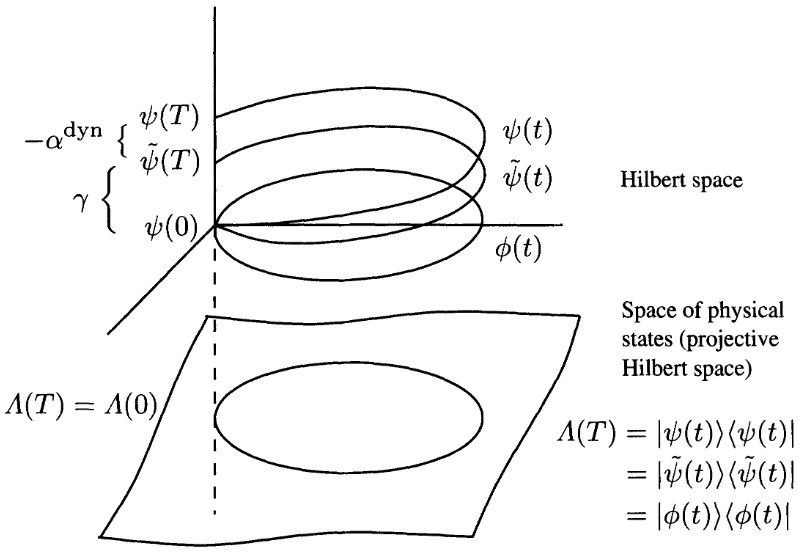
\includegraphics[width=0.7\textwidth]{fig/schéma2Bohm}
	\caption{Schéma de Bohm \cite{bohm_geometric_2003} sur les trois phases}
	\label{fig:2lifts}
\end{figure}

Quand on dit que $\Tilde{\psi}$ est l'\textit{horizontal lift}, on sous entend que le fibré est munie d'une connexion. Suivant l'approche quantique, elle est de la forme :
\[\forall \eta\in\Gamma(\mathcal{M}),\quad  \mathcal{A} \defeq \int_\gamma \big\langle \eta, h(\eta) \big\rangle\]
où $h$ est l'Hamiltonien de l'équation de Schrödinger (dont $\psi$ est supposé solution) :
\begin{equation}\label{eq:schrodinger}
	i\frac{d}{dt} \psi(t) = h\big(\psi(t)\big)
\end{equation}
Mais on a le choix de $h$. En particulier, si on veut pas de contrainte, on peut toujours poser :
\[h = i\frac{d}{dt}\]
Est-ce qu'on a le droit ? (je vois pas pourquoi on pourrait pas) Et si on le fait, qu'est-ce que ca dit du point de vue mécha Hamiltonienne ? (\apriori~rien vue l'EDP)
\\
Aussi, du pvd calculatoire / de la phase g, qu'est-ce qu'il se passe ? Typiquement, est-ce que y'a $\Tilde{\psi}$ devient un $\phi$ ?
\\

Aussi, chose remarquable, le fait que la phase géométrique soit invariante par gauge transfo réapprait dans le fait que $\phi$ ne soit pas définie à gauge tranfo près (sauf au bord). Par contre c'est étrange que 



\subsection{La vision Mukunda \& Simon \cite{mukunda_quantum_1993,mukunda_quantum_1993-1}}

\begin{itemize}
	\item Mukunda \& Simon\cite[p. 10]{mukunda_quantum_1993} partent des matrices de corrélation $\rho = \psi\psi^\dagger$ vérifiant (cas normé, p.50 pour le cas générale) :
	\begin{align*}
		\rho &= \rho^\dagger \geq 0  &  \rho^2 &= \rho  &  \tr(\rho) &= 1 (=\|\rho\|^2)
	\end{align*}
	et pose l'Hamiltonien  (resp. l'énergie kiné) :
	\begin{align*}
		H &= i\big( \dot{\psi} \psi^\dagger - \psi\dot{\psi}^\dagger - \langle \psi, \dot{\psi}\rangle\big)  &  \text{resp. }\ K &= \frac{d}{dt}\big( \psi\psi^\dagger \big) = \dot{\rho}
	\end{align*}
	qui donne :
	\[\frac{d}{dt}\psi = -i H\psi = \big( K + \langle\psi, \dot{\psi}\rangle \big)\]
	$K$ est "mieux" dans le sens où il est invariant par gauge-t. Aussi, comme c'est une dérivée d'une hermitienne elle est... hermitienne ? (mmmh).
	
	Anyway, on peut poser avec la bonne gauge :
	\[\frac{d}{dt}\Tilde{\psi} = K\Tilde{\psi}\]
	\\
	
	\item Voir page 20 pour passer de $\phaseg$ au Birgmann invar
	\\
	
	\item La phase totale $\phaset(\psi,t_0,t)$ est la phase dyn de la géodésique reliant $\psi(t)$ à $\psi(t_0)$ (ca commute ? surement pas)
	\\
	En somme, la phase totale est complètement indépendante du chemin $\psi$, ce qui est rassurant puisque c'est ce qu'on attend la phase totale : qu'elle ne compare que les états $\psi(t_0)$ et $\psi(t)$.
	
	\item L'invariant de Birgmann à des propriétés sommatoires similaires à un calcul de volume... transition parfaite vers la formule de Stokes !!!
	
	\item SUPER IMPORTANT : \cite[(8.6),p.51]{mukunda_quantum_1993} pour l'originie/choix de $\phaseg$ !
\end{itemize}







\setcounter{figure}{0}
\setcounter{lstlisting}{0}

\part{Brouillon}

\section{Intuition sur les fondamentaux}

\subsection{Réflexion autour du produit hermitien}

Soit $x,y\in\C^n$ des vecteurs complexes et $X,Y\in\R^{2\times n}$ leur versions réelles. On note $x^j$ sa $j^{eme}$ composante complèxe et $x_1$ (resp. $x_2$) le vecteur composé de ses parties réelles (resp. imaginaires) :
\[x = \big(x^j\big)_j =  x_1 + ix_2 =  \big(x^j_1\big)_j +i \big(x^j_2\big)_j\]
\\
On a deux façon d'écrire le produit hermitien (canonique) de $x$ avec $y$.
\\
La première :
\begin{align*}
\langle x,y \rangle = \langle x_1 + ix_2, y_1 + iy_2\rangle &= \langle x_1, y_1\rangle - i \langle x_1,y_2\rangle +i\langle x_2, y_1\rangle + \langle x_2, y_2\rangle  \\
&= \langle x_1, y_1\rangle + \langle x_2, y_2\rangle 
+ i\big(\langle x_2, y_1\rangle - \langle x_1,y_2\rangle\big) \\
&= \sum_j x^j_1 y^j_1+ x^j_2 y^j_2
+ i\left(\sum_j x^j_2 y^j_1 -  x^j_1y^j_2\right) \\
&= \left\langle \begin{pmatrix} x_1 \\ x_2 \end{pmatrix},\begin{pmatrix} y_1 \\ y_2 \end{pmatrix}\right\rangle
+ i\left\langle \begin{pmatrix} x_1 \\ x_2 \end{pmatrix},\begin{pmatrix} -y_2 \\ y_1 \end{pmatrix}\right\rangle \\
&= \Big\langle X,Y\Big\rangle 
+ i\left\langle X,\begin{pmatrix} 0 & -I_n \\ I_n & 0 \end{pmatrix}\begin{pmatrix} y_1 \\ y_2 \end{pmatrix}\right\rangle\\
&= \Big\langle X,Y\Big\rangle 
- i\left\langle X,\begin{pmatrix} 0 & I_n \\ -I_n & 0 \end{pmatrix}Y\right\rangle
\end{align*}
\\
Cette formule peut s’interpréter en disant que le produit hermitien encode le produit scalaire entre $X$ et $Y$ et le produit scalaire de $X$ avec les vecteurs $y^j=(y^j_1, y^j_2)$  auquel on aurait applique une rotation de $90^\circ$ (rotation qui, par ailleurs, correspond à la multiplication par $i$ dans le plan complexe). Moralement, $\langle x,y \rangle =0$ demande une orthogonalité de $X$ à un plan, ce qui fait sens puisque cela tient compte du fait que les $x^j, y^j$ sont complexes (donc de dimension 2 en tant que $\R-$e.v.).
\\
Pour les connaisseurs, on retrouve l'égalité ``produit hermitien $=$ produit scalaire $-i$ forme symplectique'' !!
Voir
\href{https://fr.wikipedia.org/wiki/Espace_projectif#Espace_projectif_complexe}{plan proj complexe} et \href{https://fr.wikipedia.org/wiki/Vari%C3%A9t%C3%A9_k%C3%A4hl%C3%A9rienne}{variété kählérienne }
\\

On a aussi l'écriture (quand-même moins clair) :
\begin{align*}
\langle x,y \rangle &= \langle x_1, y_1\rangle + \langle x_2, y_2\rangle 
+ i\big(\langle x_2, y_1\rangle - \langle x_1,y_2\rangle\big) \\
&= \sum_j x^j_1 y^j_1+ x^j_2 y^j_2+ i\sum_j \big( x^j_2 y^j_1 - x^j_1y^j_2 \big) \\
&= \sum_j \big\langle X^j,Y^j\big\rangle - i\sum_j \det(X^j, Y^j)
%&= \sum_j \|X^j\|\|Y^j\| \cos \widehat{X^j,X^j} + i\sin \widehat{X^j,Y^j}
\end{align*}
Cette formule dit que les parties reélles et imaginaires du produit $\langle x,y \rangle$ encodent respectivement ``l'orthogonalité moyenne'' et la ``linéarité moyenne ''entre les familles de vecteurs $X^j\in\R^2$ et $Y^j\in\R^2$. L'orthogonalité d'une part parce que le produit scalaire s'annule en cas d'orthogonalité (no shit), la linéarité d'autre part car le déterminant s'annule en cas de colinéarité et moyenne car se sont des sommes sur $j$. \textbf{$\bf{\langle x,y \rangle=0}$ ne dit pas que les le vecteurs sont à la fois colinéaire et orthogonaux parce que ce sont des valeurs moyennes (\ie~annuler une somme ne veut pas dire que chacun des termes sont nuls).}
\\

Si maintenant on s'intéresse au cas $y=x$, on a $\forall h\in\C^n$ :
\begin{align*}
\langle x+h, x+h \rangle = \langle x, x \rangle + \langle x, h \rangle + \langle h, x \rangle + \langle h, h \rangle 
&= \langle x, x \rangle + \langle x, h \rangle  + \congu{\langle x, h \rangle }+ \langle h, h \rangle \\
&= \langle x, x \rangle + 2\Re e \langle x, h \rangle + \langle h, h \rangle
\end{align*}
Donc si $x\in\C^n$ est fonction d'un paramètre $t$, l'égalité $\ \langle x, \dot{x} \rangle = \frac{1}{2}\partial_t\langle x, x \rangle\ $ du cas réel devient :
\begin{equation}\label{eq:x_scal_dotx}
\langle x\,|\, \dot{x} \rangle = \frac{1}{2}\partial_t\langle x\,|\, x \rangle + i\left\langle X\,´\Big|\,\begin{pmatrix} 0 & -I_n \\ I_n & 0 \end{pmatrix}\dot{X}\right\rangle
\end{equation}
\\
En particulier, quand bien-même $x$ serait de norme constante, on aurait toujours un degré de liberté pour $\ \langle x, \dot{x} \rangle$ :
\[\|x\|=c\quad \Lr\quad \langle x, \dot{x} \rangle = i\left\langle X,\begin{pmatrix} 0 & -I_n \\ I_n & 0 \end{pmatrix}\dot{X}\right\rangle\]




\section{Description des signaux multivariés}\label{sec:bases}

\subsection{Cas bivarié et trivarié}

\subsubsection{Bivarié}

\begin{itemize}
	
	\item Avec la transformation :
	\[\bf{x} \leadsto \big(e^{i\phi}, \bf{x}\bf{x}^\dagger\big)\in\U(1)\times \PC{1}-ish\]
	On a :
	\begin{align*}
		\bf{x}\bf{x}^\dagger &= \frac{1}{2}\sum_{n=1}^3 S_i(t)\sigma_i  &  \left\{\begin{aligned}
			S_0(t) &=\, ^t\bf{x}\congu{\bf{x}} = \|\bf{x}\|^2 \\
			S_1(t) &= S_0(t) \cos 2\chi(t)\cos 2\theta(t)\\
			S_2(t) &= S_0(t) \cos 2\chi(t)\sin 2\theta(t)\\
			S_3(t) &= S_0(t) \sin 2\chi(t)
		\end{aligned} \right.
	\end{align*}
	
	\item En version quaternion ($\bf{j}$ fait office de $i$) \cite{lefevre_polarization_2021} :
	\begin{equation}
		\sa{\bf{x}} = a(t)e^{\bf{i}\theta} e^{-\bf{k}\chi} e^{\bf{j}\phi}
	\end{equation}
	Et les Stokes parameters sont donnée par :
	\[\sa{\bf{x}} \bf{j} \congu{\sa{\bf{x}}} = S_0  +\bf{i}S_3 + \bf{j}S_1 + \bf{k}S_2\]
	Et le lien avec les $\sigma_i$ se fait via (mais du coup les notations colles par :/) :
	\[(\sigma_0, \sigma_1, \sigma_2, \sigma_3) \leadsto (1, \bf{i}, \bf{j}, \bf{k})\]
	
	\item Et en version matrice de Pauli :
	\begin{equation}
		\sa{\bf{x}} = a(t)e^{i\phi} e^{i\theta \sigma_2} e^{-i\chi \sigma_1} \begin{pmatrix} 1 \\ 0 \end{pmatrix}
	\end{equation}
\end{itemize}
\noindent
Plus de détail : \\ 

On a un signal bivarié $\bf{x}(t) = \big(x(t),y(t)\big)$ qu'on transforme (voir \cref{subsec:transfo_SA}) soit la forme :
\[\sa{\bf{x}}(t) = \begin{pmatrix}x_+(t) \\ y_+(t)\end{pmatrix} = \begin{pmatrix}a_x(t) e^{i\phi_x(t)} \\ a_y(t) e^{i\phi_y(t)}\end{pmatrix}\in\C^2\]
\\

\`A côté de ça, on a les ellipses modulées :
\[z(t) = e^{i\theta}\big(a(t)\cos\phi(t) + ib(t) \sin\phi(t)\big) = a(t) e^{i\theta} \big( \sin\chi(t) \cos\phi(t) + i\sin\chi(t) \sin\phi(t) \big) \in\C\]
Qui sous forme vectoriel se réécrit \textbf{(pourquoi ???)} :
\begin{equation}%\label{eq:exp_elliptik}
	z(t) = e^{i\phi(t)} R_{\theta(t)}\begin{pmatrix} a(t) \\ -ib(t) \end{pmatrix} = a(t)e^{i\phi(t)} R_{\theta(t)} \begin{pmatrix} \cos\chi(t) \\ -i\sin\chi(t) \end{pmatrix} \in\C^2,\qquad R_\theta\in\SO_2(\R) \
\end{equation}
\\

Pour avoir la désinscription de $\bf{x}$ en terme d’ellipse, il suffit donc de poser :\footnote{C'est la version analytique du la version vectorielle de l'ellipse !}
\[\sa{\bf{x}}(t) = z(t)\quad \Llr\quad \begin{pmatrix}a_x(t) e^{i\phi_x(t)} \\ a_y(t) e^ {i\phi_y(t)}\end{pmatrix} = A(t)e^{i\phi} R_{\theta(t)} \begin{pmatrix} \cos\chi(t) \\ -i\sin\chi(t) \end{pmatrix}\]
\\
Ensuite, on pose :
\[\begin{pmatrix}z_+ \\ z_-\end{pmatrix} = \begin{pmatrix}a_+ e^{i\phi_+} \\ a_- e^{i\phi_-}\end{pmatrix} = \frac{1}{2}\begin{pmatrix}x_+ + iy_+ \\ x_+ - iy_+\end{pmatrix} = \frac{1}{2}\begin{pmatrix}1 & i \\ 1 & -i\end{pmatrix} \begin{pmatrix}x_+ \\ y_+\end{pmatrix}\]
\\
Et on a :
\begin{align*}
	2\phi &= \phi_+ + \phi_-  &  a &= A\cos\chi = a_+ + a_- \\
	2\theta &= \phi_+ - \phi_-  &  b &= A\sin\chi = a_+ - a_- 
\end{align*}
et on en déduit :
\begin{align*}
	A &= \sqrt{(a_+ + a_-)^2 + (a_+ - a_-)^2}  &  \begin{aligned} \cos\chi &= \frac{a_+ + a_- }{\sqrt{(a_+ + a_-)^2 + (a_+ - a_-)^2}}  \\  \sin\chi &= \frac{a_+ - a_- }{\sqrt{(a_+ + a_-)^2 + (a_+ - a_-)^2}}	\end{aligned}
\end{align*}
Ce qui donne \infine (super osef) :
\[\begin{pmatrix}x_+ \\ y_+\end{pmatrix} = e^{i\frac{\phi_+ + \phi_-}{2}} R_{\frac{\phi_+ - \phi_-}{2}} \begin{pmatrix}a_+ + a_- \\ -i(a_+ - a_-)\end{pmatrix}\]
\\

L'\cref{eq:exp_elliptik_2var} ce généralise  très bien, il suffit d'augmenter la taille de $R_\theta\in\SO_n(\R)$ et de lui donner le vecteur étendu :\footnote{\textit{Sachant que le vecteur contenant $a$ et $b$ est principalement nul, on peut réécrire le produit ne considérant que les deux premières colonnes de $R_\theta$.}}
\[z_x(t) = \begin{pmatrix}x_{1+}(t) \\ \vdots \\ 
	x_{n+}(t)\end{pmatrix} = e^{i\phi} R_{\theta(t)}\begin{pmatrix} a(t) \\ -ib(t) \\ 0 \\ \vdots \\ 0 \end{pmatrix} = A(t)e^{i\phi} R_{\theta(t)} \begin{pmatrix} \cos\chi(t) \\ -i\sin\chi(t) \\ 0 \\ \vdots \\ 0 \end{pmatrix}\]
\\

Maintenant, la question est de savoir comment généraliser la transformation en $(z_+, z_-)$ pour obtenir les paramètres $(A, \phi, R_\theta, \chi)$ dans ce cas...
\\
Pour généraliser le procédé, on peut noter que :
\[\begin{pmatrix}z_+ \\ z_-\end{pmatrix} = \frac{1}{2}\begin{pmatrix}1 & i \\ 1 & -i\end{pmatrix} \begin{pmatrix}x_+ \\ y_+\end{pmatrix} = \frac{1}{\sqrt{2}}U \begin{pmatrix}x_+ \\ y_+\end{pmatrix}\qquad\qquad \text{avec }\ U=\frac{1}{\sqrt{2}}\begin{pmatrix}1 & i \\ 1 & -i\end{pmatrix}\in\U(2)\]
\\ 
Ce qui ramène à se demander comment généraliser $U$ à $\U(n)$. Le problème est que $U$ est indépendant de tout les paramètres $(A, \phi, R_\theta, \chi)$ et sa généralisation est vraiment pas évidente sachant qu'on que le formule avec $n=2$... et pour $n=3$ ca devient déjà chaud (pour rappelle $\dim \SO_n(\R)=\frac{n(n-1)}{2}$ et donc $\theta\in\R^n$, ce qui rend le problème de pire en pire à mesure qu'on augmente $n$).



\subsubsection{Trivarié}

\begin{itemize}
	\item Version de Lilly \cite{lilly_modulated_2011}
	\begin{equation}
		\begin{aligned}
			\sa{\bf{x}}(t) &= e^{i\phi(t)} R_1\big(\alpha(t)\big)\ R_3\big(\beta(t)\big)\ R_1\big(\theta(t)\big)\begin{pmatrix}
				a(t) \\ -ib(t) \\ 0
			\end{pmatrix} \\
			&= a(t)e^{i\phi(t)} R_1\big(\alpha(t)\big)\ R_3\big(\beta(t)\big)\ R_1\big(\theta(t)\big)\begin{pmatrix}
				\cos\chi(t) \\ -i\sin\chi(t) \\ 0
			\end{pmatrix}
		\end{aligned}
	\end{equation}
	
	\begin{align*}
		&\text{avec : }  &  
		R_1(\theta) &= \begin{pmatrix}
			1 & 0 & 0 \\ 0 & \cos\theta & -\sin\theta \\ 0 & \sin\theta & \cos\theta
		\end{pmatrix}  &  
		R_3(\theta) &= \begin{pmatrix}
			\cos\theta & -\sin\theta & 0 \\ \sin\theta & \cos\theta & 0 \\ 0 & 0 & 1 
		\end{pmatrix}
	\end{align*}
	
	Donc une amplitude / phase instantanée $A$ / $\phi$ et une polarisation instantanée d'ellipse paramétrée par $\chi$ et orientée par la rotation $R_1R_3R_1$.
	
	\item On note d'abord que (Lefevre \cite{lefevre_polarization_2021}) :
	\[\begin{pmatrix}
		\cos\chi(t) \\ -i\sin\chi(t) \\ 0
	\end{pmatrix} = \begin{pmatrix}
		\cos\chi(t) & i\sin\chi(t) & 0 \\ -i\sin\chi(t) & \cos\chi(t) & 0 \\ 0 & 0 & 1
	\end{pmatrix}\begin{pmatrix}
		1 \\ 0 \\ 0
	\end{pmatrix}\]
	Ce qui, en terme de matrice de Gall-man $(\lambda_i)$ (généralisation de la base de Pauli à $\U(3)$), devient :
	\begin{align*}
		\sa{\bf{x}}(t) &= a(t)e^{i\phi(t)} R_1\big(\alpha(t)\big)\ R_3\big(\beta(t)\big)\ R_1\big(\theta(t)\big)\begin{pmatrix}
			\cos\chi(t) \\ -i\sin\chi(t) \\ 0
		\end{pmatrix} \\
		&= a(t)e^{i\phi(t)} e^{i\alpha \lambda_7} e^{i\beta \lambda_3} e^{i\theta \lambda_7} e^{-i\chi \lambda_1}\begin{pmatrix}
			1 \\ 0 \\ 0
		\end{pmatrix}
	\end{align*}
\end{itemize}




\subsection{VRAC}

\begin{definition}[Fourier de signal multivarié]
	La transformée de Fourier ``faible'' d'un signal multivarié est définie comme la transformée de Fourier composante par composante du signal :
	\[\mathcal{F}[\bf{x}] = \Big(\mathcal{F}[x_i]\Big)_{1\leq i\leq n}\]
\end{definition}


\begin{remarque}
	En posant (suivant les notations ci-dessus) $a = \big\|(a_i)_{1\leq i\leq n}\big\|_2$, $\bf{x}$ s'écrit :
	\[\bf{x}(t) = e^{i\varphi(t)}\begin{pmatrix} a_1(t)e^{i\varphi_1(t)} \\ a_2(t)e^{i\varphi_2(t)} \\ \vdots \\ a_n(t)e^{i\varphi_n(t)}
	\end{pmatrix} = a(t)e^{i\varphi(t)}\begin{pmatrix} \alpha_1(t)e^{i\varphi_1(t)} \\ \alpha_2(t)e^{i\varphi_2(t)} \\ \vdots \\ \alpha_n(t)e^{i\varphi_n(t)} \end{pmatrix}\]
	avec $\alpha = (\alpha_i)_{1\leq i\leq n} \in \S^{n-1}$. $\alpha$ est donc définie à une rotation près et en notant cette rotation $R_\Theta$, $\psi$ s'écrit encore :
	\begin{align*}
		\bf{x}(t) &= a(t)e^{i\varphi(t)}\begin{pmatrix} e^{i\varphi_1(t)} \\ & e^{i\varphi_2(t)} \\  & & \ddots \\ & & & e^{i\varphi_n(t)}\end{pmatrix} R_\Theta\begin{pmatrix} 1 \\ 0 \\ \vdots \\ 0 \end{pmatrix}   &  \text{où }\qquad R_\Theta\begin{pmatrix} 1 \\ 0 \\ \vdots \\ 0 \end{pmatrix} = \alpha\\
		&= a(t)e^{i\varphi(t)}e^{iDiag(\varphi_i(t))} R_\Theta\begin{pmatrix} 1 \\ 0 \\ \vdots \\ 0 \end{pmatrix} = a(t)e^{i\varphi(t)}Diag\big(e^{i\varphi_i(t)}\big) R_\Theta\begin{pmatrix} 1 \\ 0 \\ \vdots \\ 0 \end{pmatrix}
	\end{align*}
\end{remarque}

\begin{itemize}
	
	\item Faudra parler des propriétés des signaux multiva un peu, genre la différence pour fourier des images et des multivarées ($\R^n\lr\R$ vs $\R\lr\R^n$)
	
	\item + quelques propriétés pour les cas SA, y'a moyen que ca soit pas inintéressant
\end{itemize}



\subsection{Mon blabla}\label{subsec:blabla}


\begin{proposition}\label{prop:quatern}
Les signaux bivariés se décrivent très simplement à l'aide des quaternions. En considérant $\{1, \bf{i},\bf{j},\bf{k}\}$ la base canonique des quaternions $\mathbb{H}$, on peut voir $\psi$ comme étant à valeur dans ${\C_{\bf{j}}}^n$ ($\C_{\bf{j}} :=\R\times \bf{j}\R$), de sorte que :
\[\forall \psi\in L^2(\R,\mathbb{H}),\ \exists a,\theta,\chi,\varphi \in\mathcal{C}(\R)\ |\quad \psi(t) = a(t)e^{\bf{i}\theta(t)}e^{-\bf{k}\chi(t)}e^{\bf{j}\varphi(t)}\]
\\
Sous cette forme, les paramètres $a$ et $\varphi$ s'interprètent respectivement comme l'amplitude et la phase instantanée du signal. Les deux paramètres restant contrôle l'ellipticité ($\chi$) et l'orientation ($\theta$) de l’ellipse de polarisation instantanée. C'est-à-dire l'ellipse que suit la signal à l'instant $t$.
\\
Dit autrement, à tout instant $t$, $\psi(t)$ est vu comme une point d'une ellipse dont la taille est caractériser par $a(t)$, l'ellipticité par $\chi(t)$ et l'orientation par $\theta(t)$. $\phi(t)$ permet lui de situer $\varphi(t)$ sur cette ellipse.
\\

\textit{Le problème de cette représentation est qu'elle se généralise mal aux signaux plus que $2-$variés et, à notre connaissant, il n'existe pas d'extensions des quaternions à de plus haute dimension. voir \cref{prop:gene_param_signal_v1,prop:gene_param_signal_v2}, \cref{eq:phase_tot,,eq:phase_dyn,eq:phase_geo}} 
\end{proposition}

Il est évident que cette représentation est présent bien plus de paramètre que nécessaire, puisse que deux devrait suffire. Pour autant, elle permet de mieux \textbf{je sais quoi mais c'est sur qu'il y'a une raison}.
\\
Si cette représentation se généralise mal parce qu'elle demanderait d'avoir une extension de $\mathbb{H}$, sont interprétations graphique, elle, se généralise très bien. Par exemple, en dimension 3, alors l'ellipse devient une ellipsoïde. L'amplitude reste de dimension 1 parce qu'elle ne fait que contrôler la taille de cet ellipsoïde, mais les autres paramètres eux doivent être de dimension 2. L'ellipsoïde à besoin de deux angles pour être orienté, possède deux degrés d'ellipticité et ces points sont déteminés par deux angles.


\begin{proposition}\label{prop:gene_param_signal_v1}
Plus généralement, tout signal multivarié $\psi$ est (\textit{devrait être}) caractérisé par quatre paramètres (donc $1+(n-1)(\frac{n}{2}-2)$ scalaires) :
\begin{align*}
	a&\in\mathcal{C}(\R,\R^+)  &  \theta&\in\mathcal{C}(\R, [-\pi/2,\pi/2]^{\frac{n(n-1)}{2}})  &  \chi&\in\mathcal{C}(\R, [-\pi/4,\pi/4]^{n-1})  &  \varphi&\in\mathcal{C}(\R, [-\pi,\pi]^{n-1})
\end{align*}	
\end{proposition}

\`A bien y réfléchir, décrire un ellipsoïde dans l'espace, c'est exactement de que font les matrices symétriques définies positives. Donc on pourrait tout à fait remplacer les informations $(a,\theta,\chi)$ par une matrice symétrique positive de dimension $n$. Il ne resterait alors plus que $\varphi$ qui, de toute façon ne devrait pas trop être lié aux autres paramètres.

Enfin, surement que si parce que y'a un monde pour $\varphi=0_\R^n$ et c'est le reste des paramètres qui fait le travail. Mais clairement c'est pas intéressant comme description. L'idée serait plutôt décrire le signal $\psi$ en minimisant les variations de $(a,\theta,\chi)$.
Ca appelle clairement à chercher que dans l'espace de Siegel mais pas seulement, parce que c'est pas juste des chemins chez Siegel qui nous intéresse.

Ou alors c'est le jeu de gauge qui fait qu'on tue $\varphi$ ? auquel cas tout les jours Siegel.
\\

\textit{BTW, les quaternions c'est fait pour décrire les rotations et c'est (quasiment) ce qu'on fait avec, donc aller chercher dans un espace de matrices pour généraliser le principe c'est pas déconnant.}
\\
\textit{D'ailleurs, vu que c'est pas exactement ce qu'on fait avec, dans quelle mesure c'est pas le cas et est-ce qu'on exploite vraiment la structure des quaternions ?}


\begin{proposition}\label{prop:gene_param_signal_v2}
Autre approche : un signal multivarié étant moralement un chemin de $\R^n$, son graphe est une variété (plongée) de dimenion 1. Sachant cela, si en chaque instant on veut définir l'ellipsoïde sur laquelle elle repose à un insant $t$, il est morale que cette ellipsoïde soit en fait une ellipse puisque c'est elle-même une variété de dimension 1.
\\
Partant de là, on aurait toujours $a$, $\chi$ et $\phi$ pour la décrire et seulement $\theta$ gagnerait en dimension pour pouvoir orienter l'ellipse dans les $n$ axes. $\psi$ serait alors la données de $3+\frac{n(n-1)}{2}$ paramètres :
\begin{align*}
	a&\in\mathcal{C}(\R,\R^+)  &  \theta&\in\mathcal{C}(\R, [-\pi,\pi]^{\frac{n(n-1)}{2}})  &  \chi&\in\mathcal{C}(\R, [-\pi/4,\pi/4])  &  \varphi&\in\mathcal{C}(\R, [-\pi,\pi])
\end{align*}
\end{proposition}

On aurait beaucoup moins de paramètre et c'est quand-même bien. En même temps ca parait plus contraignant comme modèle. Pour comparer les deux, il faudrait voir comment les deux se décomposant dans le cas d'un signal qui ne varierait sur une ellipsoïde fixe. \ie dans un cas où $\theta,\chi$ de la \cref{prop:gene_param_signal_v1} varie pas alors que ceux de la \cref{prop:gene_param_signal_v2} si.



\section{Vrac}

\subsection{Random  stuff ready pour rédac (+labeled)}

\begin{definition}[Signal multivarié]\label{def:signal_multivar}
	Un \emph{signal multivarié}, ou \emph{$n-$varié}, est un vecteur composé de $n\in\N^*$ signaux $x_i$. Si $n=2$, alors on parle de signal \emph{bivarié}.
	\\
	Dans la continuité de ce qui à été dit dans la \cref{subsec:transfo_SA}, dans le cas des signaux réels, on s'intéressera au vecteur composé des transformées en SA (eq. \ref{eq:transfo_SA}, déf. \ref{def:transfo_sa&hilbert}) des $x_i$.
	\textbf{Au moins dans toute cette \namecref{sec:sign_multivar}}, un tel signal sera noté :
	\[\sa{x}(t)\ :\quad \begin{aligned} 
		\R\quad &\lr\qquad \C^n \\t\quad &\longmapsto\ \begin{pmatrix} \mathcal{A}[x_1] \\ 
			\mathcal{A}[x_2] \\ \vdots \\ \mathcal{A}[x_n] \end{pmatrix}
	\end{aligned} \]
	On supposera que chaque composante $x_i$ de $\bf{x}$ aura autant de régularité et de condition d'intégrabilité que nécessaire \textbf{(il vaudra préciser lesquelles à un moment)}.
\end{definition}

\begin{definition}\label{def:phase_dyn}
	Ainsi, il reste tout un degré de liberté au produit $\ \langle x, \dot{x} \rangle\ $ même si $x\in\S^{2n}$. En intégrant ce degré de liberté supplémentaire, c'est-à-dire en tenant compte de son évolution sur la période $[t_0,t]$, l'on obtient ce qui est appeller le \emph{phase dynamique} :
	\[\phased \defeq \phased(t_0,t) = \int_{t_0}^t \Im m \big\langle \psi(s) \, |\, \dot{\psi}(s) \big\rangle ds\]
	Elle dynamique en cela qu'elle est propre au variation de $\psi$ et qu'elle considère tout l'évolution de $\psi$ : ça dynamique.
\end{definition}


\begin{definition}[Connexion de Berry]\label{def:berry_connx}
	On appelle \emph{connexion de Berry} le champ de forme linéaire :
	\begin{equation}\label{eq:berry_connx}
		\forall \psi\in\mathpzc{M},\quad A_\psi :\ \begin{aligned} T_\psi\mathpzc{M}\ &\lr\qquad\ \R \\ \phi\quad &\longmapsto\ \Im m \big\langle \psi(s) \, |\, \phi(s) \big\rangle
		\end{aligned}
	\end{equation}
	\textbf{Elle a rien d'une connexion par contre :/}
\end{definition}



\subsection{Bilan des formules}

\begin{itemize}
	\item Les phases de $\psi$ entre les instants $t_0$ et $t$ :
	\begin{equation}\label{eq:phase_tot}
		\phaset(\psi, t_0, t) \defeq \arg\big\langle\psi(t_0) \,|\, \psi(t)\big\rangle = \arctan \left( -\frac{\big\langle\psi(t_0), \omega\psi(t)\big\rangle}{\big\langle\psi(t_0), \psi(t)\big\rangle} \right)
	\end{equation}
	
	\begin{equation}\label{eq:phase_dyn}
		\phased(\psi,t_0,t) \defeq \Im m \int_{t_0}^t\big\langle \psi(s) \,|\, \dot{\psi}(s) \big\rangle ds
	\end{equation}
	
	\begin{equation}\label{eq:phase_geo}
		\phaseg(\psi, t_0, t) \defeq \phaset(\psi, t_0, t) - \phased(\psi,t_0,t)
	\end{equation}
	
	\item (conservative) Équation Schrödinger et de Liouville-von Neumann ($h(R)$ : Hamiltonien des paramètres $R$, $W$ : opérateurs statistique ) \cite[p.6]{bohm_geometric_2003} :
	\begin{equation}%\label{eq:schrodinger}
		i\frac{d \psi(t)}{dt} = h(R)\psi(t)
	\end{equation}
	\begin{equation}\label{eq:liouville-neumann}
		i\frac{d W(t)}{dt} = \big[h(R),W(t)\big] \qquad\qquad [\cdot\,,\cdot]=\text{ commutateur ?}
	\end{equation}
	
	\item Moment angulaire (viteuf) $\forall z\in\C$ :
	\begin{equation}\label{eq:mom_angu}
		M(t) = \Re e \big(iz\congu{z}'\big) = -\Im m z\congu{z}'  \qquad\qquad \text{thoughts ?}
	\end{equation}
	
\end{itemize}


\subsection{Thoughts}

\begin{itemize}
	\item Si la phase géo est la phase dyn - phase tot et est invariante as gauge t, est-ce que la phase tot correspond à la phase (dyn) entre $t_0$ et $t$ suivant la géodesique ?
	
	\item La ``Berry connection'' c'est une vraie connexion ? elle est où la covariance alors ?
\end{itemize}

\[\underline{\overline{\qquad\qquad\qquad\qquad\qquad\qquad\qquad\qquad\qquad\qquad\qquad\qquad\qquad\qquad\qquad\qquad\qquad\qquad}}\]{\color{white}relbinrei}

\begin{itemize}
	\item ``horizontal lift'' : pourquoi horizontal ? en quel sens ? (parce que fibré)
	
	\item Fréquence de Rubi
	
	\item Matrice/base de Pauli et généralisation, groupe $SU(n)$ (un peu de quantique ?)
	
	\item Monopole de Dirac + lien avec la phase géo (un peu d'électro-magnétisme ?)
	
	\item Invariant de Bargmann + série de Dyson
\end{itemize}


\newpage

\listoffigures
\vfill
\lstlistoflistings
\vfill
%\listtheorems

\newpage

\bibliography{ref.bib}{}
\bibliographystyle{siam}
\end{document}